\documentclass[10pt,english,aspectratio=169]{beamer}

\usepackage{ae,aecompl}
\usepackage[T1]{fontenc}
\usepackage{textcomp}
\usepackage[utf8]{inputenc}
\usepackage{babel}

\setcounter{secnumdepth}{3}
\setcounter{tocdepth}{3}

\usepackage{amsmath, amssymb, graphicx}
\usepackage{booktabs, multirow}
\usepackage{tikz}
\usetikzlibrary{positioning,arrows.meta,shapes,calc}
\usepackage{listings}
\usepackage{xcolor}
\usepackage{tcolorbox}

\lstset{
  basicstyle=\ttfamily\small,
  keywordstyle=\color{blue!80!black}\bfseries,
  commentstyle=\color{green!50!black}\itshape,
  stringstyle=\color{orange!80!black},
  backgroundcolor=\color{gray!8},
  frame=single,
  rulecolor=\color{gray!40},
  breaklines=true,
  showstringspaces=false,
  numbers=none,
}

\lstdefinestyle{pythonstyle}{
    language=Python,
    basicstyle=\ttfamily\footnotesize,
    keywordstyle=\color{blue!80!black}\bfseries,
    commentstyle=\color{green!50!black}\itshape,
    stringstyle=\color{orange!80!black},
    frame=single,
    rulecolor=\color{gray!40},
    backgroundcolor=\color{gray!8},
    breaklines=true,
    showstringspaces=false,
    numbers=left,
    numbersep=5pt,
    numberstyle=\tiny\color{gray}
}

\ifx\hypersetup\undefined
  \AtBeginDocument{%
    \hypersetup{bookmarks=false,breaklinks=true,pdfborder={0 0 0},colorlinks=true,
      linkcolor=DarkText,urlcolor=RedTitle}%
  }
\else
  \hypersetup{bookmarks=false,breaklinks=true,pdfborder={0 0 0},colorlinks=true,
    linkcolor=DarkText,urlcolor=RedTitle}%
\fi

\makeatletter
\newcommand\makebeamertitle{\frame{\maketitle}}%
\AtBeginDocument{%
  \let\origtableofcontents=\tableofcontents
  \def\tableofcontents{\@ifnextchar[{\origtableofcontents}{\gobbletableofcontents}}
  \def\gobbletableofcontents#1{\origtableofcontents}%
}

\usetheme{metropolis}
\usefonttheme{professionalfonts}

\definecolor{LightGray}{RGB}{230,230,230}
\definecolor{RedTitle}{RGB}{0,0,200}
\definecolor{VeryLightGray}{RGB}{245,245,245}
\definecolor{DarkText}{RGB}{0,0,0}

\setbeamercolor{background canvas}{bg=white}
\setbeamercolor{title}{fg=RedTitle}
\setbeamercolor{author}{fg=DarkText}
\setbeamercolor{date}{fg=DarkText}
\setbeamercolor{frametitle}{bg=VeryLightGray,fg=DarkText}
\setbeamercolor{normal text}{fg=DarkText}

\setbeamersize{text margin left=5mm, text margin right=5mm}
\addtobeamertemplate{frametitle}{}{\vspace{-0.5em}}
\newcommand{\reducevspace}{\vspace{-0.5cm}}

\setbeamertemplate{navigation symbols}{}
\setbeamertemplate{footline}{%
  \hfill%
  \usebeamercolor[fg]{page number in head/foot}%
  \usebeamerfont{page number in head/foot}%
  \insertframenumber\,/\,\inserttotalframenumber\kern1em\vskip2pt%
}

\makeatother

\graphicspath{{figures/}}


\title[ML \& Agentic AI for Macro Research]{Machine Learning and Agentic AI for Macroeconomic Research\\
9: Agentic AI and Claude Code\\[0.5em]}
\author{Zhigang Feng}
\date{Spring 2026}

\begin{document}

\makebeamertitle

%===========================================================
% AGENDA
%===========================================================

\begin{frame}{Lecture Agenda}

\begin{columns}[T]
\begin{column}{0.5\textwidth}
\begin{enumerate}
    \item What is agentic AI? (vs.\ LLM, vs.\ RAG)
    \item Claude Code: under the hood
    \item The 5-pillar workflow (detail)
    \item Tool landscape + Codex comparison
    \item The homotopy workflow
    \item The iterative workflow
    \item Project structure: \texttt{.claude/}
\end{enumerate}
\end{column}
\begin{column}{0.5\textwidth}
\begin{enumerate}
    \setcounter{enumi}{7}
    \item Beginner mistakes to avoid
    \item Skills, agents, sub-agents
    \item Tracing Aiyagari end-to-end
    \item Case studies + your first exercise
    \item How research changes + limitations
    \item Wrap-up
\end{enumerate}
\end{column}
\end{columns}

\vspace{0.4cm}

\textbf{The throughline:} the \textit{5-pillar workflow}---introduced on the next slide---is referenced on every section divider in this lecture.
\end{frame}

\begin{frame}
\frametitle{The 5-Pillar Workflow}

\begin{center}
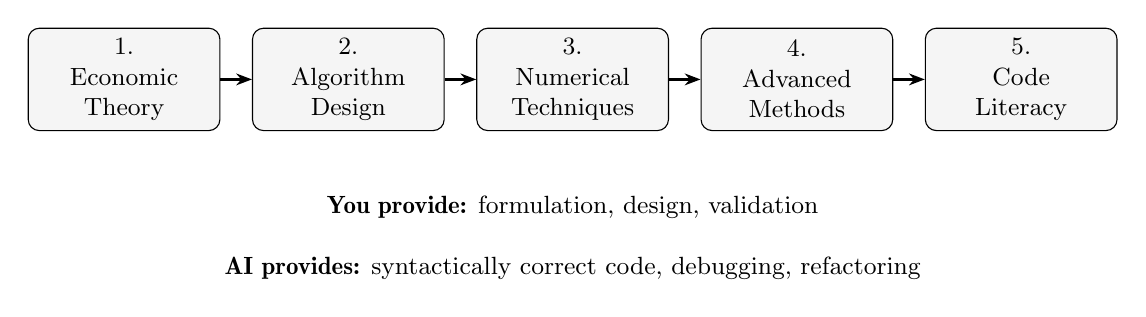
\begin{tikzpicture}[
    pillar/.style={rectangle, draw=black, fill=VeryLightGray, rounded corners,
                   minimum width=2.4cm, minimum height=1.3cm,
                   text width=2.2cm, align=center, font=\small},
    arrow/.style={-{Stealth[length=2mm]}, thick}
]
    \node[pillar] (p1) {1.\\ Economic\\Theory};
    \node[pillar, right=0.4cm of p1] (p2) {2.\\ Algorithm\\Design};
    \node[pillar, right=0.4cm of p2] (p3) {3.\\ Numerical\\Techniques};
    \node[pillar, right=0.4cm of p3] (p4) {4.\\ Advanced\\Methods};
    \node[pillar, right=0.4cm of p4] (p5) {5.\\ Code\\Literacy};

    \draw[arrow] (p1) -- (p2);
    \draw[arrow] (p2) -- (p3);
    \draw[arrow] (p3) -- (p4);
    \draw[arrow] (p4) -- (p5);

    \node[below=0.7cm of p3, font=\small] (you) {\textbf{You provide:} formulation, design, validation};
    \node[below=0.25cm of you, font=\small] {\textbf{AI provides:} syntactically correct code, debugging, refactoring};
\end{tikzpicture}
\end{center}

\vspace{0.3cm}

\textbf{This is the throughline.} Every section in this lecture comes back to one of these five pillars. Mastering them is what makes you the \textit{research architect}---AI handles the bricks; you design the structure.
\end{frame}

%===========================================================
\section{What is Agentic AI?}
%===========================================================

\begin{frame}
\frametitle{The Naive Baseline: ChatGPT in a Browser Tab}

You ask in a chat window:

\vspace{0.2cm}
\begin{center}
\textit{``Pull the FOMC meeting dates since 2008 and plot the federal-funds-rate path around each meeting.''}
\end{center}
\vspace{0.2cm}

A plain chatbot will write Python that \textit{looks} reasonable. But it cannot:

\begin{enumerate}
    \item \textbf{Execute} the code---it has no Python interpreter
    \item \textbf{Fetch} the data---it has no network or file access
    \item \textbf{Iterate} on real output---it never sees the error messages or the wrong dates
    \item \textbf{Persist} state---tomorrow it forgets your project conventions and variable names
\end{enumerate}

\vspace{0.3cm}

\textbf{The result:} you become the human shuttle---copy code into your editor, run it, copy the error back, paste the new code, repeat. \textit{This is what we are about to fix.}
\end{frame}

\begin{frame}
\frametitle{Chatbot $\to$ RAG $\to$ Agent: a Capability Spectrum}

\textbf{One question across all three:} \textit{``Plot the federal-funds-rate path around recent FOMC meetings.''}

\vspace{0.4cm}

\begin{center}
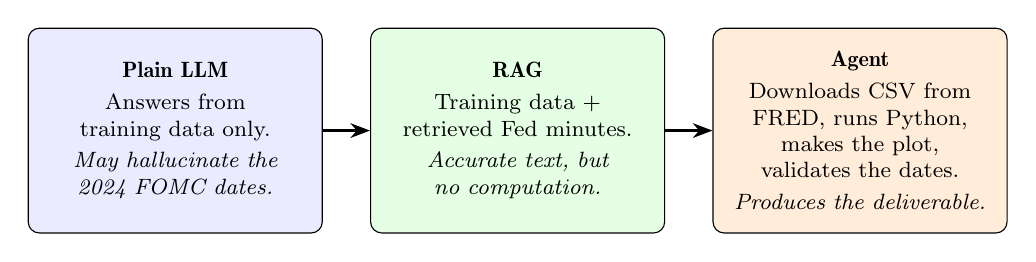
\begin{tikzpicture}[
    box/.style={rectangle, draw=black, rounded corners,
                minimum width=3.7cm, minimum height=2.6cm,
                text width=3.5cm, align=center, font=\footnotesize},
    arrow/.style={-{Stealth[length=2.5mm]}, thick}
]
    \node[box, fill=blue!8] (llm) {\textbf{Plain LLM}\\[2pt]
        Answers from training data only.\\[2pt]
        \textit{May hallucinate the 2024 FOMC dates.}};
    \node[box, fill=green!10, right=0.6cm of llm] (rag) {\textbf{RAG}\\[2pt]
        Training data + retrieved Fed minutes.\\[2pt]
        \textit{Accurate text, but no computation.}};
    \node[box, fill=orange!15, right=0.6cm of rag] (agent) {\textbf{Agent}\\[2pt]
        Downloads CSV from FRED, runs Python, makes the plot, validates the dates.\\[2pt]
        \textit{Produces the deliverable.}};

    \draw[arrow] (llm) -- (rag);
    \draw[arrow] (rag) -- (agent);
\end{tikzpicture}
\end{center}

\vspace{0.3cm}

\textbf{Each step adds capability without removing anything.} An agent \textit{contains} an LLM and can call retrieval; the spectrum is cumulative. You will use all three in a single research project.
\end{frame}

\begin{frame}
\frametitle{What Makes Something ``Agentic''?}

Four defining features---each illustrated with an empirical-economics example:

\vspace{0.3cm}

\begin{itemize}
    \item \textbf{Tool use}: invokes \texttt{pandas}, \texttt{curl}, \texttt{R}, \texttt{statsmodels}, the shell---whatever the task requires
    \vspace{0.1cm}
    \item \textbf{Autonomy}: plans a multi-step empirical workflow without re-prompting
    \begin{itemize}
        \item \textit{e.g.,} ``download FRED $\to$ clean $\to$ regress $\to$ plot $\to$ save table'' as one command
    \end{itemize}
    \vspace{0.1cm}
    \item \textbf{Iteration}: observes that a regression failed, identifies the bad column, fixes the formula, reruns
    \vspace{0.1cm}
    \item \textbf{Persistence}: remembers your project conventions across sessions (variable naming, preferred packages, validated benchmarks)
\end{itemize}

\vspace{0.3cm}

\textbf{All four features are cumulative.} Tool use without autonomy = a glorified Python REPL. Autonomy without iteration = a script that runs once and dies on the first error. You need all four for ``agentic.''
\end{frame}

\begin{frame}[fragile]
\frametitle{The Bridge: How a Chatbox Becomes a Terminal Agent}

\textbf{One key technical change:} modern LLMs (post-2023) support \textbf{structured tool calls}.
Instead of writing ``you should run \texttt{python solve.py},'' the model emits a machine-readable request:

\begin{lstlisting}[style=pythonstyle,language={},basicstyle=\ttfamily\scriptsize,numbers=none]
{ "tool": "Bash", "command": "python aiyagari_v0.py" }
\end{lstlisting}

A \textbf{harness}---software installed on your Mac---executes this and returns the real output. The model reads it and decides what to do next. This loop is what makes something ``agentic.''

\vspace{0.2cm}

\begin{center}
\small
\begin{tabular}{|l|c|c|}
\hline
& \textbf{claude.ai (browser)} & \textbf{Claude Code (terminal)} \\ \hline
LLM model & \multicolumn{2}{c|}{same (Opus 4.6)} \\ \hline
Harness & none (sandboxed) & local CLI on your Mac \\ \hline
Can run Python? & no & yes---\textit{your} Python, \textit{your} machine \\ \hline
Sees real errors? & no & yes---loops back automatically \\ \hline
\end{tabular}
\end{center}

\vspace{0.2cm}

\textbf{Same brain, different arms.} The terminal agent is not a smarter model---it is the \textit{same} model given real tools. The harness is what flips the switch from text-only to text\,+\,actions.
\end{frame}

\begin{frame}
\frametitle{Standalone LLM vs.\ RAG vs.\ Agent}

\begin{center}
\small
\begin{tabular}{|p{2.4cm}|p{2.7cm}|p{2.9cm}|p{4.2cm}|}
\hline
& \textbf{Plain LLM} & \textbf{LLM + RAG} & \textbf{Agent} \\ \hline
\textbf{Knowledge source} & Training data & Training + retrieved docs & Training + retrieved docs + live data fetched at runtime \\ \hline
\textbf{Action capability} & None (text only) & None (text only) & Reads/writes files, runs code, hits APIs \\ \hline
\textbf{State persistence} & Per-conversation & Per-conversation & Cross-session via files \\ \hline
\textbf{Latency} & Seconds & Seconds & Minutes (multi-step) \\ \hline
\textbf{Typical economic use} & Brainstorming model setup & Literature review of Fed minutes & Full empirical pipeline (FRED $\to$ figure) \\ \hline
\end{tabular}
\end{center}

\vspace{0.3cm}

\textbf{Different tools for different stages.} You will use all three in a single research project: an LLM to design the model, RAG to find relevant papers, an agent to run the regression and make the figure.
\end{frame}

\begin{frame}
\frametitle{The Ladder of AI Coding Maturity}

\begin{center}
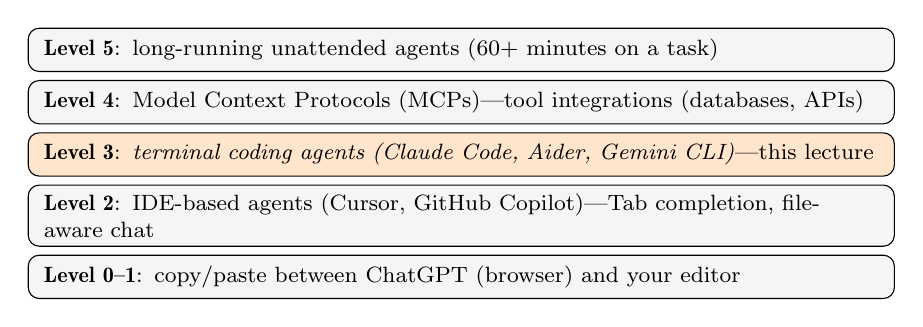
\begin{tikzpicture}[
    rung/.style={rectangle, draw=black, fill=VeryLightGray, rounded corners,
                 minimum width=11cm, minimum height=0.55cm,
                 text width=10.6cm, align=left, font=\footnotesize},
]
    \node[rung] (l0) {\textbf{Level 0--1}: copy/paste between ChatGPT (browser) and your editor};
    \node[rung, above=0.1cm of l0] (l2) {\textbf{Level 2}: IDE-based agents (Cursor, GitHub Copilot)---Tab completion, file-aware chat};
    \node[rung, above=0.1cm of l2, fill=orange!20] (l3) {\textbf{Level 3}: \textit{terminal coding agents (Claude Code, Aider, Gemini CLI)}---this lecture};
    \node[rung, above=0.1cm of l3] (l4) {\textbf{Level 4}: Model Context Protocols (MCPs)---tool integrations (databases, APIs)};
    \node[rung, above=0.1cm of l4] (l5) {\textbf{Level 5}: long-running unattended agents (60+ minutes on a task)};
\end{tikzpicture}
\end{center}

\vspace{0.3cm}

\textbf{Where most economists are today:} Level 1--2.\\
\textbf{Where this lecture takes you:} Level 3.

\vspace{0.2cm}

\textit{Adapted from Paul Goldsmith-Pinkham, ``Getting Started with Claude Code.''}
\end{frame}

\begin{frame}
\frametitle{Why Level 3 is the Sweet Spot for Empirical Research}

At Level 3 you get \textbf{tool use + autonomy + iteration}, but you still stay in the loop to validate.

\vspace{0.3cm}

\begin{itemize}
    \item \textbf{Below Level 3} (browser chat / Cursor) \\
    Too manual: you re-explain the project every session; the AI never sees its own output
    \vspace{0.15cm}
    \item \textbf{Level 3} (Claude Code) \\
    Right balance: the AI runs the code, sees real errors, fixes them---but a human approves each major step
    \vspace{0.15cm}
    \item \textbf{Above Level 3} (long-running unattended agents) \\
    Too risky for research code: nobody is watching when the agent silently changes a regression specification or grid choice
\end{itemize}

\vspace{0.3cm}

\textbf{Concrete example:} a single Aiyagari V0 $\to$ V1 $\to$ V2 cycle---design $\to$ implement $\to$ validate $\to$ extend---is exactly the kind of bounded, validated task that Level 3 was built for.
\end{frame}

\begin{frame}
\frametitle{Claude Code in Context: Alternatives}

Claude Code is one of several Level-3 terminal agents. Each has a similar architecture:

\vspace{0.3cm}

\begin{center}
\small
\begin{tabular}{|l|p{9.5cm}|}
\hline
\textbf{Tool} & \textbf{One-line description} \\ \hline
\textbf{Claude Code} & Anthropic's terminal agent. Largest context window. Strong reasoning. Used for the rest of this lecture \\ \hline
\textbf{Gemini CLI} & Google's terminal agent. Free tier with Gemini Pro. Tight Google-services integration \\ \hline
\textbf{OpenAI Codex CLI} & OpenAI's terminal agent. Tight ChatGPT-Plus integration \\ \hline
\textbf{Aider} & Open-source terminal agent. Bring-your-own model (Claude / GPT / local). Good git integration \\ \hline
\textbf{Cursor} (Level 2) & Most popular IDE-integrated agent. Tab completion + chat + multi-file composer \\ \hline
\end{tabular}
\end{center}

\vspace{0.3cm}

\textbf{The workflow we teach transfers to any Level-3 agent.} We use Claude Code as the concrete example because the file-based harness (\texttt{CLAUDE.md}, \texttt{.claude/}) is the best documented and most stable.
\end{frame}

\begin{frame}
\frametitle{Codex vs.\ Claude Code: A Budget-Aware Comparison}

Panjwani's (2026) recommendation for economists starting today on a tight budget: \textbf{start with Codex.}

\vspace{0.2cm}

\begin{center}
\small
\begin{tabular}{|l|p{5.0cm}|p{5.0cm}|}
\hline
& \textbf{OpenAI Codex} & \textbf{Claude Code} \\ \hline
\textbf{Model (2026)} & GPT 5.4 & Claude Opus 4.6 \\ \hline
\textbf{\$20/mo tier} & Higher usable throughput & More restrictive rate limits \\ \hline
\textbf{Desktop app} & Polished GUI for most users & Terminal-native (power users) \\ \hline
\textbf{Context window} & Shorter & Largest available (\textasciitilde200K tokens) \\ \hline
\textbf{Harness files} & \texttt{AGENTS.md}, \texttt{.agents/skills/} & \texttt{CLAUDE.md}, \texttt{.claude/skills/} \\ \hline
\end{tabular}
\end{center}

\vspace{0.2cm}

\textbf{Important caveat:} \textit{``This space changes fast---today it's Codex, tomorrow it's back to Claude, the day after something else.''} The recommendation is for \textit{this moment}, not permanent truth.

\vspace{0.1cm}

\textit{Source: Panjwani (2026). He has switched back and forth between the two tools over time.}
\end{frame}

\begin{frame}
\frametitle{Skills Are an Open Standard}

You are \textbf{not} locked into an ecosystem. The workflow concepts transfer cleanly:

\vspace{0.3cm}

\begin{center}
\small
\begin{tabular}{|l|l|l|}
\hline
\textbf{Concept} & \textbf{Claude Code} & \textbf{Codex} \\ \hline
Project context file & \texttt{CLAUDE.md} & \texttt{AGENTS.md} \\ \hline
Skills directory & \texttt{.claude/skills/} & \texttt{.agents/skills/} \\ \hline
Rules directory & \texttt{.claude/rules/} & \texttt{.agents/rules/} \\ \hline
Agent definitions & \texttt{.claude/agents/} & \texttt{.agents/agents/} \\ \hline
\end{tabular}
\end{center}

\vspace{0.3cm}

\textbf{What this means in practice:}
\begin{itemize}
    \item A colleague's skill written for Codex works in Claude Code with minimal adaptation
    \item If you switch tools next month, your project harness migrates with you
    \item The \textit{workflow}---plan first, encode skills, validate against benchmarks---is tool-agnostic
\end{itemize}

\vspace{0.2cm}

\textbf{This reinforces the main claim:} the workflow we teach in this lecture transfers to \textit{any} Level-3 agent. Learn the pattern, not the brand.
\end{frame}

%===========================================================
\section{Claude Code: Under the Hood}
%===========================================================

\begin{frame}
\frametitle{Three Components of Claude Code}

Claude Code has three physically distinct parts:

\vspace{0.2cm}

\begin{columns}[T]
\begin{column}{0.55\textwidth}
\begin{enumerate}
    \item \textbf{The Harness} (lives on your Mac)\\
    \small CLI software you install. Reads your files, runs shell commands, manages the conversation loop. This is what ``Claude Code'' means when installed.

    \vspace{0.2cm}

    \item \textbf{The LLM} (lives on Anthropic's servers)\\
    \small Every message is bundled with conversation history and sent via HTTPS to the API. The ``thinking'' happens in the cloud.

    \vspace{0.2cm}

    \item \textbf{Your Files} (live on your Mac)\\
    \small Python scripts, data CSVs, LaTeX---all on your disk. Code executes on your hardware with your packages.
\end{enumerate}
\end{column}
\begin{column}{0.4\textwidth}
\begin{center}
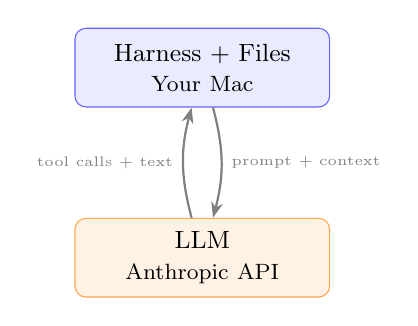
\begin{tikzpicture}[
    macbox/.style={rectangle, draw=blue!60, fill=blue!8, rounded corners,
                   minimum width=3.2cm, minimum height=1.0cm,
                   text width=3.0cm, align=center, font=\small},
    cloudbox/.style={rectangle, draw=orange!70, fill=orange!10, rounded corners,
                     minimum width=3.2cm, minimum height=1.0cm,
                     text width=3.0cm, align=center, font=\small},
    arrow/.style={-{Stealth[length=2mm]}, thick, gray}
]
    \node[macbox] (harness) {Harness + Files\\{\footnotesize Your Mac}};
    \node[cloudbox, below=1.4cm of harness] (llm) {LLM\\{\footnotesize Anthropic API}};
    \draw[arrow, bend left=15] (harness) to node[right,font=\tiny] {prompt + context} (llm);
    \draw[arrow, bend left=15] (llm) to node[left,font=\tiny] {tool calls + text} (harness);
\end{tikzpicture}
\end{center}
\vspace{0.3cm}
\footnotesize
\textbf{Key:} code runs locally.\\
Only the \textit{conversation} traverses the network. Your data never uploads.
\end{column}
\end{columns}
\end{frame}

\begin{frame}
\frametitle{The Mac File Hierarchy: Global vs.\ Local}

Two layers of configuration. \textbf{Local overrides global.}

\vspace{0.2cm}

\begin{center}
\footnotesize
\begin{tabular}{|l|l|p{5.5cm}|}
\hline
\textbf{Path} & \textbf{Scope} & \textbf{What lives here} \\ \hline
\texttt{\textasciitilde/.claude/settings.json} & Global & Default permissions, model preference \\ \hline
\texttt{\textasciitilde/.claude/MEMORY.md} & Global & Cross-project memory (persists forever) \\ \hline
\texttt{\textasciitilde/.claude/skills/} & Global & Skills available in every project \\ \hline
\hline
\texttt{<project>/CLAUDE.md} & Local & Project brain, read every session \\ \hline
\texttt{<project>/.claude/settings.json} & Local & Project permissions (overrides global) \\ \hline
\texttt{<project>/.claude/skills/} & Local & This project's slash commands \\ \hline
\texttt{<project>/.claude/agents/} & Local & Specialized reviewer roles \\ \hline
\texttt{<project>/.claude/rules/} & Local & Always-on guardrails \\ \hline
\end{tabular}
\end{center}

\vspace{0.2cm}

\textbf{On a Mac:} \texttt{\textasciitilde} = \texttt{/Users/yourname}. To see what you have: \texttt{ls \textasciitilde/.claude/}

\vspace{0.1cm}

\textbf{Practical rule:} global \texttt{\textasciitilde/.claude/} is your personal defaults (apply everywhere). Local \texttt{.claude/} is the project's rules (apply only here). Set permissions you always want globally; set project-specific conventions locally.
\end{frame}

\begin{frame}
\frametitle{Initialization: What Happens When You Type \texttt{claude}}

Five steps run \textbf{before you type your first message}:

\vspace{0.2cm}

\begin{enumerate}
    \item \textbf{Read global config} \\
    Loads \texttt{\textasciitilde/.claude/settings.json}: permission defaults, model preference

    \vspace{0.1cm}

    \item \textbf{Detect project context} \\
    Searches current directory (and parents) for \texttt{CLAUDE.md} and \texttt{.claude/}

    \vspace{0.1cm}

    \item \textbf{Load project brain} \\
    Reads \texttt{CLAUDE.md} into the context window---Claude now ``knows'' the project

    \vspace{0.1cm}

    \item \textbf{Auto-load all rules} \\
    Every \texttt{.claude/rules/*.md} file is loaded silently---no action required from you

    \vspace{0.1cm}

    \item \textbf{Ready} \\
    Context window is pre-populated with project knowledge before you say anything
\end{enumerate}

\vspace{0.25cm}

\textbf{Analogy:} step 4 is a professor re-reading lecture notes before class. Students arrive; context is already loaded.

\vspace{0.1cm}

\textbf{Cost warning:} steps 3--4 consume tokens before you type anything. Keep \texttt{CLAUDE.md} and rules files concise.
\end{frame}

\begin{frame}[fragile]
\frametitle{The Permission System and Local Code Execution}

\begin{columns}[T]
\begin{column}{0.44\textwidth}
\textbf{Claude's toolbox:}

\vspace{0.15cm}
\footnotesize
\begin{tabular}{|l|p{2.8cm}|}
\hline
\textbf{Tool} & \textbf{What it does} \\ \hline
\texttt{Bash} & Run any shell command \\ \hline
\texttt{Read} & Read a file from disk \\ \hline
\texttt{Write} & Create or overwrite a file \\ \hline
\texttt{Grep/Glob} & Search content / find files \\ \hline
\texttt{Agent} & Spawn a child Claude instance \\ \hline
\end{tabular}
\end{column}
\begin{column}{0.53\textwidth}
\textbf{The permission model:}

\vspace{0.1cm}
\footnotesize
\begin{itemize}
    \item \textbf{Default:} Claude asks before every Bash call. You see the exact command before it runs.
    \item \textbf{Whitelist:} add trusted commands to \texttt{.claude/settings.json}:
\end{itemize}
\begin{lstlisting}[style=pythonstyle,language={},basicstyle=\ttfamily\tiny,numbers=none]
"allowedTools": [
  "Bash(python *)",
  "Bash(git *)"  ]
\end{lstlisting}
\begin{itemize}
    \item \textbf{Bypass-permissions:} skips all prompts. Use only when you fully trust the task.
\end{itemize}
\end{column}
\end{columns}

\vspace{0.2cm}

\textbf{``Which Python ran this?'' (common confusion):}
\begin{itemize}
    \item Claude's Bash inherits your shell's \texttt{\$PATH}
    \item If you ran \texttt{conda activate myenv} before \texttt{claude}, \textit{that} Python runs---not a special Anthropic Python
    \item To confirm: add a \texttt{which python} check to your \texttt{CLAUDE.md} conventions
\end{itemize}
\end{frame}

\begin{frame}
\frametitle{Key Modes: Plan, Effort, and Session Control}

\begin{center}
\footnotesize
\begin{tabular}{|l|p{5.0cm}|p{3.3cm}|}
\hline
\textbf{Command / Key} & \textbf{What it does} & \textbf{When to use} \\ \hline
\texttt{Shift+Tab} & \textbf{Plan mode}: Claude writes a plan, does NOT execute. Waits for your approval. & Start every non-trivial task here \\ \hline
\texttt{/effort max} & Maximum reasoning depth: highest quality, slower, costs more & Novel problems, economic correctness \\ \hline
\texttt{/effort default} & Balanced quality and speed & Routine edits, simple queries \\ \hline
\texttt{/cost} & Show tokens used + estimated USD for this session & Budget check before long tasks \\ \hline
\texttt{Esc} & Interrupt Claude mid-task immediately & When it's going the wrong way \\ \hline
\texttt{/compact} & Summarize conversation to free context window & After \textasciitilde{}20 turns; between phases \\ \hline
\texttt{/clear} & Wipe context, start fresh & New unrelated task \\ \hline
\end{tabular}
\end{center}

\vspace{0.2cm}

\textbf{The effort--cost tradeoff:}
\begin{itemize}
    \item \texttt{/effort max} + long context $\approx$ \$5--15 per complex session (Opus 4.6 pricing)
    \item Spend effort on \textit{decisions}: algorithm choice, debugging wrong economics, code review
    \item Save effort on \textit{execution}: renaming variables, reading files, small edits
\end{itemize}
\end{frame}

%===========================================================
\section{The 5-Pillar Workflow (Detail)}
%===========================================================

\begin{frame}
\frametitle{Pillar 1: Economic Theory}

You must \textbf{formulate the economic problem precisely}:

\vspace{0.2cm}

\textbf{Household optimization:}
\begin{itemize}
    \item Write the objective: $\max \mathbb{E}_0 \sum_{t=0}^\infty \beta^t u(c_t, n_t)$
    \item Specify constraints: budget, borrowing limits, information structure
    \item Derive optimality conditions: Euler equations, transversality
\end{itemize}

\textbf{Equilibrium concepts:}
\begin{itemize}
    \item Define competitive equilibrium: optimality + market clearing
    \item Recursive competitive equilibrium for computation
    \item Partial vs.\ general equilibrium
\end{itemize}

\vspace{0.3cm}

\textbf{Aiyagari anchor:} \textit{Without a precisely written household problem (CRRA utility, asset state, borrowing constraint), the AI's Aiyagari code may solve a subtly different model---and you will only catch it if you wrote down the equations first.}
\end{frame}

\begin{frame}
\frametitle{Pillar 2: Algorithm Design}

You must know \textbf{how to translate theory into computation}:

\vspace{0.2cm}

\textbf{Dynamic programming approach:}
\begin{itemize}
    \item Bellman equation: $V(s) = \max_a \{u(s,a) + \beta \mathbb{E}[V(s')]\}$
    \item Value function iteration (VFI): iterate $T(V) \to V^*$ until convergence
    \item Policy function iteration (PFI): faster convergence, more complex per step
\end{itemize}

\textbf{Euler-equation methods:}
\begin{itemize}
    \item Time iteration on Euler equations directly
    \item Endogenous grid method (EGM): invert Euler equation for speed
\end{itemize}

\vspace{0.3cm}

\textbf{Aiyagari anchor:} \textit{The AI may default to grid VFI when EGM would be 50$\times$ faster on the same model. Only you know that EGM is the right call for a CRRA-utility household with a binding borrowing constraint.}
\end{frame}

\begin{frame}
\frametitle{Pillar 3: Numerical Techniques}

You must understand \textbf{how computation works} and where it breaks:

\vspace{0.2cm}

\textbf{Core techniques:}
\begin{itemize}
    \item \textbf{Optimization}: grid search, Newton methods, choice of solver for FOCs
    \item \textbf{Interpolation}: linear, cubic spline, Chebyshev---accuracy vs.\ speed
    \item \textbf{Discretization}: Tauchen, Rouwenhorst for AR(1); grid design
    \item \textbf{Simulation}: Monte Carlo for moments, ergodic distributions
\end{itemize}

\textbf{Common issues you must recognize:}
\begin{itemize}
    \item Occasionally binding constraints (borrowing limits, irreversibility)
    \item Curse of dimensionality
    \item Interpolation errors near kinks in policy functions
\end{itemize}

\vspace{0.2cm}

\textbf{Aiyagari anchor:} \textit{An AI-written Aiyagari with too few grid points near the borrowing constraint produces wrong precautionary savings. The code runs, the numbers look fine, the economics is wrong.}
\end{frame}

\begin{frame}
\frametitle{Pillar 4: Advanced Numerical Methods}

For larger or more complex models, you need \textbf{advanced solution techniques}:

\vspace{0.2cm}

\textbf{Perturbation methods:}
\begin{itemize}
    \item Linear approximation around steady state (1st order)
    \item Higher-order for welfare, risk premia (2nd, 3rd order)
    \item Fast but local---accuracy degrades far from steady state
\end{itemize}

\textbf{Projection methods:}
\begin{itemize}
    \item Global approximation using basis functions (Chebyshev, finite elements)
    \item Handles nonlinearities and occasionally binding constraints
    \item Computationally intensive, requires careful convergence checks
\end{itemize}

\vspace{0.3cm}

\textbf{Empirical anchor:} \textit{Smets-Wouters at the zero lower bound needs global methods (the ZLB binds and perturbation ignores it). The AI defaults to perturbation because it is fast. You must override this when the model has a kink.}
\end{frame}

\begin{frame}
\frametitle{Pillar 5: Code Literacy + Division of Labor}

You must \textbf{read code well enough to verify it implements your design}.

\vspace{0.2cm}

\begin{center}
\small
\begin{tabular}{|p{5.4cm}|p{6.0cm}|}
\hline
\textbf{You provide (Foundations)} & \textbf{AI provides (Implementation)} \\ \hline
Research question and model & Syntactically correct code \\ \hline
Algorithm choice and design & Translation to Python/Julia/etc.\ \\ \hline
Numerical method selection & Optimization, interpolation routines \\ \hline
Convergence/accuracy criteria & Diagnostic outputs and plots \\ \hline
Knowledge of the data and how it is set up & Data loading and cleaning \\ \hline
Economic interpretation of results & Debugging and refactoring \\ \hline
\end{tabular}
\end{center}

\vspace{0.2cm}

\textbf{You are the architect.} AI writes code; you verify it implements what you designed and validate that the answers make economic sense. Without code literacy you cannot validate; without validation, AI output is worthless.
\end{frame}

%===========================================================
\section{Tool Landscape}
%===========================================================

\begin{frame}
\frametitle{Tool 1: Chatbox (Claude.ai) --- Strengths $\to$ Workflow}

\textbf{Strengths:}
\begin{itemize}
    \item Large context window---can ingest papers, code, and detailed specs together
    \item Strong mathematical and economic reasoning
    \item Can discuss trade-offs (``Should I use VFI or EGM here?'')
\end{itemize}

\vspace{0.2cm}

\textbf{Workflow:}
\begin{enumerate}
    \item Upload paper PDF or paste model description
    \item Ask Claude to derive Bellman equation, propose algorithm, identify pitfalls
    \item Iterate on the design \textit{in chat} until you are confident
    \item Hand the polished design off to Claude Code for implementation
\end{enumerate}

\vspace{0.2cm}

\textbf{Aiyagari anchor:} \textit{design the Bellman equation and Tauchen discretization in chat \textbf{before} you ever open Claude Code.} Chatbox is the architect's whiteboard.
\end{frame}

\begin{frame}
\frametitle{Tool 2: IDE Integration (Cursor) --- Strengths $\to$ Workflow}

\textbf{Strengths:}
\begin{itemize}
    \item AI inside your editor, with full file context
    \item Tab completion as you type
    \item Multi-file edits via natural-language composer
    \item Fast feedback loop (no terminal context switch)
\end{itemize}

\vspace{0.2cm}

\textbf{Workflow:}
\begin{enumerate}
    \item Open the file you are editing
    \item Use Tab completion for boilerplate (loops, plotting, function signatures)
    \item Use chat for ``why is this loop slow?''-type questions
    \item Use composer for ``vectorize this VFI'' multi-line edits
\end{enumerate}

\vspace{0.2cm}

\textbf{Empirical anchor:} \textit{filling out a regression specification with Tab completion---you type \texttt{model = sm.OLS(}, Cursor suggests the rest based on the columns it sees in your DataFrame.}

\vspace{0.1cm}

\textit{(Full keybindings list: see Appendix~A.)}
\end{frame}

\begin{frame}
\frametitle{Tool 3: Autonomous Agent (Claude Code) --- Strengths $\to$ Workflow}

\textbf{Strengths:}
\begin{itemize}
    \item Reads and writes multiple files across your project
    \item Runs code, observes errors, debugs autonomously
    \item Spawns specialized sub-agents in parallel for review
    \item Persists context across sessions via \texttt{CLAUDE.md}
\end{itemize}

\vspace{0.2cm}

\textbf{Workflow:}
\begin{enumerate}
    \item Specify the task (English or slash command)
    \item Claude plans, gets approval, then implements
    \item Verify, review, fix loop runs autonomously
    \item You inspect the result and provide corrections (which become memory)
\end{enumerate}

\vspace{0.2cm}

\textbf{Aiyagari anchor:} \textit{convert a 600-line MATLAB Aiyagari codebase to Python overnight.} You wake up to working Python with a session log explaining each design choice.

\vspace{0.05cm}

\textit{(Cross-link: alternatives in slide ``Claude Code in Context.'')}
\end{frame}

%===========================================================
\section{The Homotopy Workflow}
%===========================================================

\begin{frame}
\frametitle{Start Here: The Recommended Workflow for New Users}

\begin{columns}[T]
\begin{column}{0.52\textwidth}
\small
\begin{enumerate}
    \item[\textbf{0.}] \textbf{Before Claude---pen~+~paper}\\
    Write one sentence: \textit{``I want to [compute X] using [method Y] for [question Z].''} If you cannot write this, Claude cannot help yet.

    \vspace{0.1cm}

    \item[\textbf{1.}] \textbf{Enter plan mode (\texttt{Shift+Tab})}\\
    Describe your goal. Claude drafts a plan. \textit{Nothing runs yet.}

    \vspace{0.1cm}

    \item[\textbf{2.}] \textbf{Review and approve}\\
    Read the plan. Ask questions. Revise. Type ``approved.'' \textit{This 2-minute step saves 20 minutes of debugging.}

    \vspace{0.1cm}

    \item[\textbf{3.}] \textbf{Implement}\\
    Claude executes the approved plan. Watch permission prompts. Press \texttt{Esc} to stop if wrong.

    \vspace{0.1cm}

    \item[\textbf{4.}] \textbf{Review output}\\
    Does it make economic sense? Re-derive one number by hand.

    \vspace{0.1cm}

    \item[\textbf{5.}] \textbf{Iterate}\\
    Fix, extend one feature, compact context $\to$ return to step~1.
\end{enumerate}
\end{column}
\begin{column}{0.44\textwidth}
\begin{center}
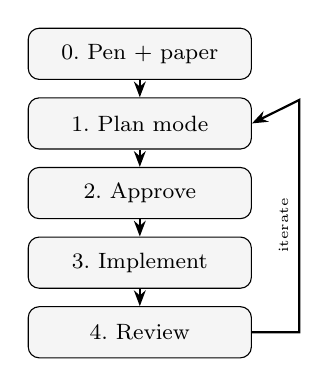
\begin{tikzpicture}[
    stagebox/.style={rectangle, draw=black, fill=VeryLightGray, rounded corners,
                 minimum width=2.8cm, minimum height=0.65cm,
                 text width=2.6cm, align=center, font=\footnotesize},
    arrow/.style={-{Stealth[length=2mm]}, thick}
]
    \node[stagebox] (s0) {0.\ Pen + paper};
    \node[stagebox, below=0.22cm of s0] (s1) {1.\ Plan mode};
    \node[stagebox, below=0.22cm of s1] (s2) {2.\ Approve};
    \node[stagebox, below=0.22cm of s2] (s3) {3.\ Implement};
    \node[stagebox, below=0.22cm of s3] (s4) {4.\ Review};
    \draw[arrow] (s0) -- (s1);
    \draw[arrow] (s1) -- (s2);
    \draw[arrow] (s2) -- (s3);
    \draw[arrow] (s3) -- (s4);
    \draw[arrow] (s4.east) -- ++(0.6,0) -- ++(0,2.95) -- (s1.east);
    \node[right=0.4cm of s3, font=\tiny, rotate=90] {iterate};
\end{tikzpicture}
\end{center}
\vspace{0.2cm}
\footnotesize
\textbf{Most common beginner mistake:} skipping Step~0. Without a clear goal, Claude will confidently build the wrong thing.
\end{column}
\end{columns}
\end{frame}

\begin{frame}
\frametitle{The Homotopy Approach to AI-Assisted Macro Research}

\textbf{From numerical methods:} homotopy continuation starts from a problem with a known solution and continuously deforms toward the target problem. The same principle applies to AI-assisted coding.

\vspace{0.3cm}

\begin{center}
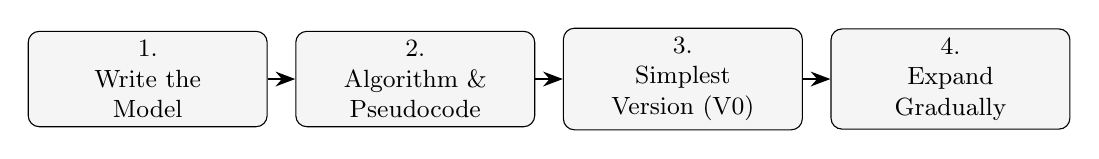
\begin{tikzpicture}[
    hstep/.style={rectangle, draw=black, fill=VeryLightGray, rounded corners,
                  minimum width=3.0cm, minimum height=1.1cm,
                  text width=2.8cm, align=center, font=\small},
    arrow/.style={-{Stealth[length=2.5mm]}, thick}
]
    \node[hstep] (s1) {1.\\Write the\\Model};
    \node[hstep, right=0.35cm of s1] (s2) {2.\\Algorithm \&\\Pseudocode};
    \node[hstep, right=0.35cm of s2] (s3) {3.\\Simplest\\Version (V0)};
    \node[hstep, right=0.35cm of s3] (s4) {4.\\Expand\\Gradually};

    \draw[arrow] (s1) -- (s2);
    \draw[arrow] (s2) -- (s3);
    \draw[arrow] (s3) -- (s4);
\end{tikzpicture}
\end{center}

\vspace{0.3cm}

\textbf{The principle:} do not ask the AI ``solve my model.'' Instead, \textit{build context incrementally}---model first, algorithm second, simple version third, extensions last. Each step gives the AI more validated context to build on.

\vspace{0.2cm}

\textbf{Why ``homotopy''?} Just as numerical homotopy traces a smooth path from a solvable problem to the target, this workflow traces a smooth path from a \textit{specifiable} model to a \textit{validated} codebase.
\end{frame}

\begin{frame}
\frametitle{Step 1: Give the AI Enough Context}

\textbf{Before any code:} write down your research question and model in \LaTeX\ or Markdown.

\vspace{0.2cm}

\textbf{What to write down:}
\begin{itemize}
    \item The research question in one sentence
    \item The full optimization problem: objective, constraints, information structure
    \item Equilibrium definition (if applicable)
    \item Parameter choices and their economic motivation
    \item What the output should look like (policy functions, distributions, moments)
\end{itemize}

\vspace{0.2cm}

\textbf{Aiyagari anchor:}
\[
\max \;\mathbb{E}_0 \sum_{t=0}^{\infty} \beta^t u(c_t) \quad \text{s.t.} \quad c_t + a_{t+1} = (1+r)a_t + w z_t, \quad a_{t+1} \geq \underline{a}
\]
with $z_t$ following a Markov chain, $u(c) = c^{1-\sigma}/(1-\sigma)$, $\sigma=2$, $\beta=0.96$.

\vspace{0.2cm}

\textbf{Why this matters:} the quality of the code the AI writes is \textit{directly proportional} to the quality of your specification. A vague prompt produces a model that looks right but solves the wrong problem. A precise specification is a contract between you and the AI.
\end{frame}

\begin{frame}
\frametitle{Step 1 in Practice: The Specification Document}

Save this as \texttt{model\_spec.md} or \texttt{model\_spec.tex} in your project folder. The AI reads it at the start of every session.

\vspace{0.2cm}

\textbf{A minimal specification for the Aiyagari model:}

\begin{enumerate}
    \item \textbf{Household problem:} CRRA utility, discount factor $\beta = 0.96$, risk aversion $\sigma = 2$
    \item \textbf{Income process:} AR(1) in logs, $\rho = 0.9$, $\sigma_\varepsilon = 0.2$, discretized via Tauchen with 7 states
    \item \textbf{Asset grid:} 200 points, triple-exponential spacing near $\underline{a}$
    \item \textbf{Solution method:} VFI with Howard improvement (50 Howard steps every 25 VFI iterations)
    \item \textbf{Convergence:} sup-norm on value function $< 10^{-8}$
    \item \textbf{Equilibrium:} $r$ clears the asset market; bisection on $r$
    \item \textbf{Output:} policy functions $c(a,z)$, $a'(a,z)$; stationary distribution $\mu(a,z)$; Gini coefficient
\end{enumerate}

\vspace{0.2cm}

\textbf{Make sure the AI understood:} ask it to restate the model in its own words before proceeding. Misunderstandings caught here cost minutes; misunderstandings caught in V2 cost hours.
\end{frame}

\begin{frame}[fragile]
\frametitle{Step 2: Algorithm and Pseudocode}

\textbf{Once the model is clear:} work with the AI on the algorithm design. Write pseudocode together---this catches design errors \textit{before} implementation.

\vspace{0.2cm}

\textbf{Aiyagari anchor---pseudocode for V0 (deterministic):}
\begin{lstlisting}[style=pythonstyle,language={},basicstyle=\ttfamily\tiny,numbers=none]
Initialize: asset grid a[1..N], guess V_old = u(r*a + w) / (1-beta)
Repeat until ||V_new - V_old|| < tol:
    For each a_i in grid:
        For each a' in grid s.t. c = (1+r)*a_i + w - a' > 0:
            compute u(c) + beta * interp(V_old, a')
        V_new[i] = max over a'
        a_policy[i] = argmax a'
    Every 25 iterations: run 50 Howard improvement steps
Return V_new, a_policy, c_policy = (1+r)*a + w - a_policy
\end{lstlisting}

\vspace{0.15cm}

\textbf{What this step produces:}
\begin{itemize}
    \item Agreement on the solution method (VFI vs.\ EGM vs.\ perturbation)
    \item Pseudocode that serves as a \textit{contract}---you and the AI agree on the algorithm before any Python is written
    \item Explicit convergence criterion and grid construction
\end{itemize}

\vspace{0.1cm}

\textbf{The AI may suggest EGM is faster.} Good---but \textit{you} decide. This is Pillar 2 (Algorithm Design) in action.
\end{frame}

\begin{frame}
\frametitle{Step 3: Start Simple --- The V0 Version}

\textbf{Implement the simplest version} of the model that captures the core structure. Debug, test, validate against analytical benchmarks. \textbf{Do NOT move on until V0 passes all benchmarks.}

\vspace{0.3cm}

\textbf{Aiyagari anchor:} V0 = deterministic income ($z_t = 1$ always).

\vspace{0.2cm}

\textbf{Three analytical benchmarks for V0:}
\begin{enumerate}
    \item $\beta(1+r) = 1$: constant consumption; $a'(a) = a$ (45-degree line)
    \item $\beta(1+r) < 1$: agent decumulates; $a \to \underline{a}$
    \item $\beta(1+r) > 1$: agent accumulates; $a$ grows without bound
\end{enumerate}

\vspace{0.2cm}

\textbf{If V0 fails these benchmarks:} the Bellman equation is wrong, the grid is broken, or the convergence criterion is too loose. \textit{Everything downstream will be wrong too.}

\vspace{0.2cm}

\textbf{The discipline:} resist the temptation to skip ahead. A working V0 takes 30 minutes. Debugging a broken V2 because V0 was never validated takes a full day.
\end{frame}

\begin{frame}
\frametitle{Step 4: Expand Gradually Until Baseline}

\textbf{Add one feature at a time.} Each expansion must have its own benchmark.

\vspace{0.3cm}

\begin{center}
\small
\begin{tabular}{|c|l|l|}
\hline
\textbf{Version} & \textbf{What you add} & \textbf{Benchmark} \\ \hline
V0 & Deterministic income & 3 analytical cases above \\ \hline
V1 & Markov income risk & Set $\sigma_z = 0$: must recover V0 exactly \\ \hline
V2 & Stationary distribution & $\sum \mu(a,z) = 1$; mass at $\underline{a}$ \\ \hline
V3 & General equilibrium & $r$ clears asset market; Gini $\approx$ data \\ \hline
\end{tabular}
\end{center}

\vspace{0.3cm}

\textbf{This IS the homotopy:}
\begin{itemize}
    \item V0 is the ``easy problem'' with a known solution
    \item Each version continuously deforms toward the research target
    \item Each validated version is the \textit{foundation} for the next
    \item If V2 breaks, you know the bug is in V2's new code---not in V0 or V1
\end{itemize}

\vspace{0.2cm}

\textbf{When to stop:} when you reach the baseline model your research question requires. The path V0 $\to$ V1 $\to$ \ldots $\to$ baseline is your audit trail.
\end{frame}

\begin{frame}
\frametitle{Why Homotopy Works with AI}

\textbf{Four reasons this workflow is especially effective with AI agents:}

\vspace{0.3cm}

\begin{enumerate}
    \item \textbf{AI excels at well-specified, bounded tasks.} ``Solve my model'' fails. ``Implement V0 per this pseudocode and validate against these 3 benchmarks'' succeeds
    \vspace{0.15cm}
    \item \textbf{Starting simple gives both you and the AI a working codebase.} V1 inherits validated V0 code. The AI has concrete, tested functions to build on---not a blank file
    \vspace{0.15cm}
    \item \textbf{Bug attribution is immediate.} If V2 breaks, the bug is in V2's new code. You and the AI can focus on the 30 new lines, not the 300 inherited ones
    \vspace{0.15cm}
    \item \textbf{Context builds naturally.} By V3, the AI has seen the model specification, the pseudocode, three validated versions, and all the corrections you made along the way. It has \textit{deep context}---not because you dumped a 10-page prompt, but because you built it incrementally
\end{enumerate}

\vspace{0.3cm}

\textbf{The numerical-methods analogy:} just as homotopy continuation avoids local optima by tracing a smooth path from a known solution, incremental model-building avoids cascading bugs by validating at every step.
\end{frame}

%===========================================================
\section{The Iterative Workflow}
%===========================================================

\begin{frame}
\frametitle{The Five-Step Loop}

\begin{center}
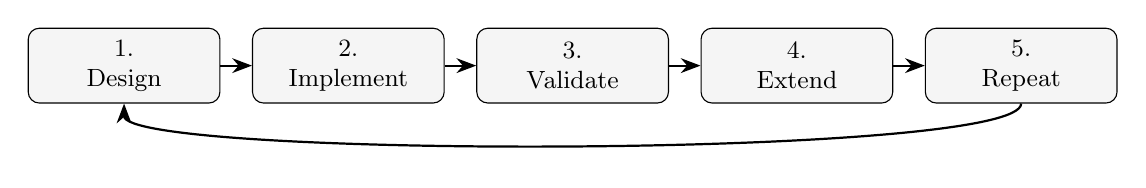
\begin{tikzpicture}[
    box/.style={rectangle, draw=black, fill=VeryLightGray, rounded corners,
                minimum width=2.4cm, minimum height=0.95cm,
                text width=2.2cm, align=center, font=\small},
    arrow/.style={-{Stealth[length=2.5mm]}, thick}
]
    \node[box] (design)   {1.\\Design};
    \node[box, right=0.4cm of design]   (impl)    {2.\\Implement};
    \node[box, right=0.4cm of impl]     (val)     {3.\\Validate};
    \node[box, right=0.4cm of val]      (ext)     {4.\\Extend};
    \node[box, right=0.4cm of ext]      (rep)     {5.\\Repeat};

    \draw[arrow] (design) -- (impl);
    \draw[arrow] (impl)   -- (val);
    \draw[arrow] (val)    -- (ext);
    \draw[arrow] (ext)    -- (rep);
    \draw[arrow] (rep.south) .. controls +(0,-0.7) and +(0,-0.7) .. (design.south);
\end{tikzpicture}
\end{center}

\vspace{0.3cm}

\textbf{Step 1: Design.} Specify state space, Bellman equation, solution method, convergence criterion. \textbf{Check extensibility} before any code.

\textbf{Step 2: Implement.} Translate algorithm to code with diagnostics (convergence plots, Euler residuals).

\textbf{Step 3: Validate.} Technical \textit{and} economic checks (next slide).

\textbf{Step 4: Extend.} Add \textit{one} feature; update design \textit{before} coding.

\textbf{Step 5: Repeat.} Each validated version is the foundation for the next.

\vspace{0.1cm}

\textbf{Pillar reference:} steps 1, 4 = Pillars 1--4. Steps 2, 3 = Pillar 5.
\end{frame}

\begin{frame}
\frametitle{Why This Workflow Works}

\textbf{1.~Separating design from implementation catches conceptual errors early.}\\
Algorithm bugs are cheaper to fix on paper than in code. Design first, implement second.

\vspace{0.3cm}

\textbf{2.~Clear attribution of bugs.}\\
Adding one feature at a time means you know exactly what caused any new issue. If V1 broke after adding income risk, you know it is the new code, not the old VFI.

\vspace{0.3cm}

\textbf{3.~AI succeeds with structured, well-specified instructions.}\\
Good communication makes good collaboration. Vague requests produce vague code.

\vspace{0.3cm}

\textbf{4.~Analytical benchmarks catch errors early.}\\
The simplest version often has closed-form solutions. Validating against these catches fundamental errors before complexity obscures them.
\end{frame}

\begin{frame}
\frametitle{Effective Prompting: Vague vs.\ Specific}

\begin{columns}[T]
\begin{column}{0.45\textwidth}
\textbf{\textcolor{red!70!black}{Vague (won't work)}}

\vspace{0.2cm}

\textit{``Analyze this data.''}

\vspace{0.4cm}

\textit{``Make it faster.''}

\vspace{0.4cm}

\textit{``Fix the regression.''}

\vspace{0.4cm}

\textit{``Add some validation.''}
\end{column}
\begin{column}{0.55\textwidth}
\textbf{\textcolor{green!50!black}{Specific (works)}}

\vspace{0.2cm}

\textit{``Load \texttt{employment.csv}, compute monthly growth rates by sector, plot a time series in BLS style.''}

\vspace{0.2cm}

\textit{``Vectorize the inner VFI loop using NumPy broadcasting; profile before/after.''}

\vspace{0.2cm}

\textit{``In the OLS, cluster standard errors at the firm level using \texttt{statsmodels}.''}

\vspace{0.2cm}

\textit{``Add an Euler-residual check; report max and mean below $10^{-6}$.''}
\end{column}
\end{columns}

\vspace{0.3cm}

\textbf{The pattern:} say \textit{exactly} which file, which variables, which package, which acceptance criterion. Verbosity is cheap; vagueness is expensive.

\textit{Source: Paul Goldsmith-Pinkham, ``Getting Started with Claude Code.''}
\end{frame}

\begin{frame}
\frametitle{Validation: Your Core Responsibility}

AI writes code. \textbf{You validate economics.} At every iteration:

\vspace{0.2cm}

\begin{columns}
\begin{column}{0.48\textwidth}
\textbf{Technical Checks}
\begin{itemize}
    \item Convergence achieved?
    \item No NaN/Inf values?
    \item Policy not hitting grid boundaries?
    \item Euler residuals small? ($<10^{-6}$)
    \item Standard errors finite?
\end{itemize}
\end{column}
\begin{column}{0.48\textwidth}
\textbf{Economic Checks}
\begin{itemize}
    \item Results economically sensible?
    \item Comparative statics correct?
    \item Limiting cases recover benchmarks?
    \item Matches analytical solutions?
    \item Magnitudes match prior beliefs?
\end{itemize}
\end{column}
\end{columns}

\vspace{0.4cm}

\textbf{Trust but verify.} AI catches indexing errors and numerical issues; \textit{you} catch economic nonsense. AI suggests diagnostics; you run them and report back.

\vspace{0.1cm}

\textbf{The boundary:} if you cannot validate a result, you cannot defend it in a seminar---and the AI cannot defend it for you.
\end{frame}

%===========================================================
\section{Project Structure}
%===========================================================

\begin{frame}
\frametitle{Naive Baseline: Chatting Without a Harness}

What happens if you just open Claude Code in an empty folder and start chatting?

\vspace{0.3cm}

\textbf{Four failure modes:}
\begin{enumerate}
    \item \textbf{You re-explain your project conventions every session.} ``Use NumPy not lists, set seed 42, use my variable naming\ldots''
    \vspace{0.1cm}
    \item \textbf{Claude forgets the correction you gave yesterday.} You corrected the asset grid bug; tomorrow it makes the same mistake.
    \vspace{0.1cm}
    \item \textbf{Every Aiyagari extension reverts to grid-VFI defaults}---ignoring your decision to use EGM, because the decision was never written down.
    \vspace{0.1cm}
    \item \textbf{No audit trail of which decisions were made why.} Six months later you cannot remember why you used Tauchen with 7 states instead of Rouwenhorst with 5.
\end{enumerate}

\vspace{0.3cm}

\textbf{The harness fixes all four.} Files on disk are how Claude remembers, learns, and stays consistent across sessions. The next 6 slides walk through what those files are.
\end{frame}

\begin{frame}[fragile]
\frametitle{What a Claude Code Project Looks Like}

\begin{lstlisting}[style=pythonstyle,language={},basicstyle=\ttfamily\tiny]
my-aiyagari-project/
+-- CLAUDE.md                    # Project brain (read every session)
+-- MEMORY.md                    # Corrections: [LEARN:tag] entries
+-- .claude/
|   +-- settings.json            # Permissions for Python, git, etc.
|   +-- skills/                  # Workflows you invoke (/command)
|   |   +-- solve-model/         #   /solve-model aiyagari v0
|   |   |   +-- SKILL.md         #   Workflow steps
|   |   |   +-- references/      #   Algorithm specs and benchmarks
|   |   |       +-- aiyagari-guide.md
|   |   +-- validate/            #   /validate aiyagari v1
|   |       +-- SKILL.md
|   +-- agents/                  # Specialized reviewers
|   |   +-- code-reviewer.md     #   Code quality, vectorization
|   |   +-- domain-reviewer.md   #   Economic correctness
|   |   +-- verifier.md          #   Runs code, checks output
|   +-- rules/                   # Standards (always active)
|       +-- plan-first-workflow.md
|       +-- orchestrator-protocol.md
|       +-- iterative-workflow.md
|       +-- verification-protocol.md
|       +-- code-conventions.md
+-- scripts/                     # Python code (aiyagari_v0.py, ...)
+-- output/                      # Figures, tables, results
+-- quality_reports/plans/       # Plans and session logs
\end{lstlisting}

\textbf{Every component you'll see for the next 10 slides has a place in this tree.}
\end{frame}

\begin{frame}[fragile]
\frametitle{CLAUDE.md --- The README for AI}

\texttt{CLAUDE.md} is read at the start of every Claude Code session.

\begin{lstlisting}[style=pythonstyle,language={},basicstyle=\ttfamily\tiny]
# CLAUDE.md --- Aiyagari Model Project
**Project:** AI & ML for Quant Macro
**Language:** Python (NumPy/SciPy)
**Philosophy:** Never skip validation between versions.

## Available Skills
| /solve-model aiyagari  | Iterative model-building workflow  |
| /validate aiyagari v1  | Run benchmarks and convergence     |

## Available Agents
| code-reviewer   | READ-ONLY | Vectorization, stability     |
| domain-reviewer | READ-ONLY | Equations, equilibrium       |
| verifier        | EXECUTE   | Runs scripts, checks output  |

## Model Versions
v0: Deterministic savings  |  v1: Income risk  |  v2: Stationary dist
\end{lstlisting}

\textbf{Python analogy:} \texttt{CLAUDE.md} $\approx$ \texttt{\_\_init\_\_.py} + \texttt{pyproject.toml}.
\end{frame}

\begin{frame}[fragile]
\frametitle{MEMORY.md --- Persistent Corrections}

\texttt{MEMORY.md} accumulates lessons learned across sessions. Each entry is a one-paragraph correction with a tag.

\begin{lstlisting}[style=pythonstyle,language={},basicstyle=\ttfamily\scriptsize]
# MEMORY.md --- Accumulated Learnings

[LEARN:aiyagari-grid] Asset grid should use more points
  near the borrowing constraint. Triple-exponential
  spacing with 200 points. Linear grids need 500+.

[LEARN:vfi-howard] Howard improvement cuts VFI iterations
  by ~80%. After every 25 VFI iterations, run 50 Howard
  steps. Convergence tolerance: 1e-8 on sup-norm.

[LEARN:notation] Convention: V for value function,
  c_pol for consumption policy, a_pol for savings policy,
  Pi for transition matrix, mu for stationary distribution.
\end{lstlisting}

\vspace{0.1cm}

\textbf{How an entry is created:} you correct Claude (``the grid is too coarse near the constraint''). Claude saves a \texttt{[LEARN:tag]} entry. Next session, it reads these \textit{before} starting work---and never repeats the mistake.
\end{frame}

\begin{frame}
\frametitle{The Three Layers: Skills, Agents, Rules}

\begin{center}
\small
\begin{tabular}{|l|c|c|c|}
\hline
& \textbf{Rules} & \textbf{Skills} & \textbf{Agents} \\ \hline
\textbf{Location} & \texttt{.claude/rules/} & \texttt{.claude/skills/} & \texttt{.claude/agents/} \\ \hline
\textbf{Loaded} & Auto, always & On \texttt{/cmd} & When skill/rule references \\ \hline
\textbf{Purpose} & \textit{How} to behave & \textit{What} to do & \textit{Who} does sub-task \\ \hline
\textbf{Mechanism} & Claude obeys & Claude follows steps & Claude reads \& adopts \\ \hline
\textbf{Python $\approx$} & Linter / config & Function & Class definition \\ \hline
\textbf{Example} & ``plan first'' & \texttt{/solve-model} & \texttt{code-reviewer.md} \\ \hline
\end{tabular}
\end{center}

\vspace{0.3cm}

\textbf{The causal chain:}
\begin{enumerate}
    \item Rules load at session start---constrain everything
    \item You invoke a skill (or give plain English)
    \item The active workflow says ``use the code-reviewer agent''---Claude reads the agent file and follows the checklist
\end{enumerate}

\vspace{0.1cm}

\textbf{Direction of control is one-way:} rules $\to$ skills $\to$ agents. Agents do \textit{not} choose skills.
\end{frame}

\begin{frame}
\frametitle{English Instructions vs.\ Encoded \texttt{SKILL.md}}

\textbf{Confusion to clear up:} What do you say in English vs.\ what is in \texttt{SKILL.md}? When does each apply?

\vspace{0.3cm}

\begin{columns}[T]
\begin{column}{0.48\textwidth}
\textbf{Plain English (one-off)}

\vspace{0.15cm}

\textit{``Implement the Aiyagari model with idiosyncratic income risk and a Tauchen-discretized AR(1) process.''}

\vspace{0.3cm}

\textbf{When to use:}
\begin{itemize}
    \item First time approaching a model
    \item Exploring an idea
    \item One-off analysis you don't expect to redo
\end{itemize}
\end{column}
\begin{column}{0.48\textwidth}
\textbf{Slash command (encoded skill)}

\vspace{0.15cm}

\texttt{/solve-model aiyagari v1}

\vspace{0.3cm}

\textbf{When to use:}
\begin{itemize}
    \item You have a workflow you want to repeat exactly
    \item Validation steps must run identically each time
    \item Multiple students or co-authors must follow the same procedure
\end{itemize}
\end{column}
\end{columns}

\vspace{0.3cm}

\textbf{Both work; the difference is reproducibility.} English is for exploration; encoded skills are for production.
\end{frame}

%===========================================================
\section{Beginner Mistakes to Avoid}
%===========================================================

\begin{frame}
\frametitle{Mistake 1: Treating Git as Optional}

\textbf{Memorable line from Panjwani (2026):} \textit{``You don't need to know Git to use Git.''}

\vspace{0.3cm}

\textbf{Three reasons Git matters for agentic workflows:}

\begin{enumerate}
    \item \textbf{Safe experimentation.} Git lets you try changes and roll them back. Without Git, every agent experiment is \textit{irreversible}---one bad refactor and your working code is gone
    \vspace{0.1cm}
    \item \textbf{Agent memory.} Once your project has real commit history, the agent can inspect how files evolved---it can reason about when a bug was introduced by reading \texttt{git log} and \texttt{git diff}
    \vspace{0.1cm}
    \item \textbf{Parallel work.} Git worktrees let you work on multiple aspects of a project simultaneously---the agent can restructure code on one branch while you continue analysis on another
\end{enumerate}

\vspace{0.3cm}

\textbf{Practical step:} put this line in your \texttt{CLAUDE.md} or \texttt{AGENTS.md}:

\vspace{0.1cm}

\begin{center}
\texttt{``Make atomic git commits as you go along.''}
\end{center}

\vspace{0.1cm}

\textit{Source: Panjwani (2026). See also: ``Why Git Makes Claude Code 10$\times$ More Powerful'' (ai-mba.io).}
\end{frame}

\begin{frame}
\frametitle{Mistake 2: Underutilizing Skills}

\textbf{Skills = saved playbooks.} Instead of re-explaining everything each session, you invoke the skill and the agent starts with context.

\vspace{0.3cm}

\textbf{Economists have repeatable tasks:}
\begin{itemize}
    \item Review a paper (argument structure, econometric spec, citation completeness)
    \item Run a data-analysis workflow (load $\to$ EDA $\to$ regress $\to$ publication tables)
    \item Prepare a funding proposal (donor profile, context brief, draft)
    \item Work with Stata or Beamer in project-specific ways
    \item Summarize meeting notes or seminar feedback
\end{itemize}

\vspace{0.3cm}

\textbf{Without skills:} you re-explain the same workflow every session---the same failure mode as ``chatting without a harness'' (see Section~6). Claude interprets ``validate'' differently each time.

\vspace{0.2cm}

\textbf{With skills:} methodology is on disk, version-controlled, and shareable with co-authors. Your workflow becomes \textit{reproducible infrastructure}, not ephemeral chat.
\end{frame}

\begin{frame}
\frametitle{Economist-Authored Skills in the Wild}

Three real examples from working economists---not toy demos:

\vspace{0.3cm}

\textbf{1.\ Pedro Sant'Anna's \texttt{review-paper} skill:}
\begin{itemize}
    \item Reads the full manuscript end-to-end
    \item Evaluates across 6 dimensions (argument, econometrics, citations, \ldots)
    \item Generates 3--5 ``referee objections'' and saves to \texttt{quality\_reports/}
\end{itemize}

\vspace{0.15cm}

\textbf{2.\ Pedro Sant'Anna's \texttt{data-analysis} skill:}
\begin{itemize}
    \item End-to-end R workflow: setup $\to$ EDA $\to$ main analysis $\to$ publication-ready tables and figures
\end{itemize}

\vspace{0.15cm}

\textbf{3.\ Chris Blattman's \texttt{proposal-write} skill:}
\begin{itemize}
    \item Drafts funding proposals from structured inputs
    \item Auto-gathers project context, builds donor profile, produces a polished draft
\end{itemize}

\vspace{0.2cm}

\textbf{Sources:} \texttt{github.com/pedrohcgs/claude-code-my-workflow}; \texttt{github.com/chrisblattman/claudeblattman}

\vspace{0.1cm}

\textbf{Key point:} treat these as \textit{patterns to adapt}, not scripts to install blindly. Your workflow is unique---customize.
\end{frame}

\begin{frame}
\frametitle{Mistake 3: One Giant Thread (Context Pollution)}

\textbf{The symptom:} ``Codex got dumber'' or ``Claude got dumber'' after 30 turns.

\vspace{0.2cm}

\textbf{The real problem:} \textit{context pollution}, not model collapse. A long thread mixes planning, implementation, debugging, and revision. The context window fills with stale intermediate thoughts that are no longer relevant---but the model still pays attention to them.

\vspace{0.3cm}

\textbf{The fix---a two-session workflow:}
\begin{enumerate}
    \item \textbf{Plan session:} discuss the design, iterate on the approach, reach agreement
    \item \textbf{Write plan to a file:} save the agreed plan as \texttt{plan.md}
    \item \textbf{Fresh execution session:} start a new conversation and execute only the plan
\end{enumerate}

\vspace{0.3cm}

\textbf{Why this works:} the execution session's context window is entirely available for implementation. No stale planning artifacts, no abandoned debug logs, no 15-turn-old constraint that the model has forgotten.

\vspace{0.2cm}

\textbf{Cross-link:} this connects directly to the \texttt{/compact} strategy in the ``Context Window Mechanics'' slides---both are about \textit{protecting the context window for the work that matters now}.
\end{frame}

%===========================================================
\section{Skills, Agents, Sub-agents}
%===========================================================

\begin{frame}
\frametitle{Naive Baseline: Why Encode Workflows at All?}

What if you just type the workflow steps in English every session?

\vspace{0.3cm}

\textbf{Four failure modes:}
\begin{enumerate}
    \item \textbf{You forget step 4 the third time.} Last week you remembered to run Euler residuals; this week you don't.
    \vspace{0.1cm}
    \item \textbf{Claude interprets ``validate'' differently each time.} Once it means convergence checks; once it means a comparison plot; once it means a unit test. Inconsistent.
    \vspace{0.1cm}
    \item \textbf{No version control on your methodology.} If your workflow improves, the improvement lives in your head, not in a file you can diff.
    \vspace{0.1cm}
    \item \textbf{Impossible to reproduce a colleague's approach.} Your co-author has a different mental workflow---now you have two methodologies and no source of truth.
\end{enumerate}

\vspace{0.3cm}

\textbf{Skills fix all four}---by writing the methodology to disk, once, in a place Claude reads every time.
\end{frame}

\begin{frame}
\frametitle{Skills = Callable Workflows}

A \textbf{skill} is a multi-step workflow invoked by name---like a Python function.

\vspace{0.2cm}

\begin{columns}
\begin{column}{0.45\textwidth}
\textbf{Python function:}
\begin{itemize}
    \item Defined once, called by name
    \item Takes arguments
    \item Executes a defined sequence
    \item Calls other functions/classes
\end{itemize}
\end{column}
\begin{column}{0.5\textwidth}
\textbf{Claude Code skill:}
\begin{itemize}
    \item Defined in \texttt{SKILL.md}
    \item Invoked: \texttt{/skillname arg}
    \item Follows step-by-step instructions
    \item References agent files by name
\end{itemize}
\end{column}
\end{columns}

\vspace{0.3cm}

\textbf{Aiyagari example:}
\[
\texttt{/solve-model aiyagari v1}
\]
runs the same 5-step methodology every time: design $\to$ implement $\to$ verify $\to$ review $\to$ score. The methodology is in \texttt{SKILL.md}; you do not retype it.

\vspace{0.2cm}

\textbf{Skills are the glue.} Rules constrain behavior; agents define roles; \textit{skills} sequence them into a workflow.
\end{frame}

\begin{frame}
\frametitle{Skill File Structure}

A skill lives in \texttt{.claude/skills/[name]/} with a required \texttt{SKILL.md}:

\vspace{0.3cm}

\begin{center}
\ttfamily
\begin{tabular}{l}
.claude/skills/solve-model/ \\
\quad $\vdash$ SKILL.md \quad\quad\quad\quad\quad\; (required: workflow steps) \\
\quad $\llcorner$ references/ \quad\quad\quad\quad\; (optional: detailed guides) \\
\quad\quad\quad $\vdash$ aiyagari-guide.md \; (Aiyagari algorithm details) \\
\quad\quad\quad $\llcorner$ rbc-guide.md \quad\;\;\; (RBC algorithm details) \\
\end{tabular}
\end{center}

\vspace{0.3cm}

\normalfont
\textbf{SKILL.md} has two parts:
\begin{enumerate}
    \item \textbf{YAML frontmatter}: name, description, command, arguments
    \item \textbf{Markdown body}: workflow steps, validation criteria, prompting patterns
\end{enumerate}

\vspace{0.2cm}

\textbf{Reference files} contain detailed model-specific algorithms. Claude loads them \textit{only when needed}, keeping the context window efficient.
\end{frame}

\begin{frame}
\frametitle{Agents = Role Descriptions, Not a Dispatch System}

An \textbf{agent file} is a markdown document describing a specialized role---its checklist, review criteria, and report format. Claude Code does \textbf{not} have a native agent dispatcher.

\vspace{0.15cm}

\textbf{What actually happens:}
\begin{enumerate}
    \item A skill (or always-on rule) says: ``spawn the code-reviewer agent''
    \item Claude reads \texttt{.claude/agents/code-reviewer.md}
    \item Claude either (a) adopts the role itself in the current conversation, or (b) launches a subagent via the Task tool---a separate Claude instance
\end{enumerate}

\vspace{0.15cm}

\textbf{Three Aiyagari agents:}
\begin{itemize}
    \item \texttt{code-reviewer.md}: vectorization, NumPy broadcasting, no hardcoded paths
    \item \texttt{domain-reviewer.md}: Euler-equation correctness, equilibrium consistency
    \item \texttt{verifier.md}: actually runs \texttt{aiyagari\_v1.py}, checks convergence
\end{itemize}

\vspace{0.1cm}

\textbf{Why separate files?} A single prompt asking about all three dimensions does a mediocre job at each. Separation enables focus.
\end{frame}

\begin{frame}
\frametitle{Subagents = Parallel Child Processes}

When Claude launches a subagent, it spawns a \textbf{separate Claude instance} with its own context window.

\vspace{0.3cm}

\begin{itemize}
    \item Multiple subagents can run \textbf{in parallel}, like Python's \texttt{multiprocessing}
    \item Each receives the agent file as its prompt
    \item Each runs to completion and returns a report
    \item The main conversation receives the reports and decides what to do
\end{itemize}

\vspace{0.3cm}

\textbf{Aiyagari example:} after writing \texttt{aiyagari\_v1.py}, the orchestrator spawns:
\begin{center}
\texttt{code-reviewer} \quad \textbf{$\Vert$} \quad \texttt{domain-reviewer}
\end{center}
in parallel. Both finish in roughly the same wall-clock time it took one to run sequentially. \textbf{Review time is halved.}

\vspace{0.2cm}

\textbf{Python analogy:} \texttt{multiprocessing.Pool().map(review, [code, domain])}.
\end{frame}

\begin{frame}
\frametitle{Rules = Always-On Guardrails}

\textbf{Rules} are the only component that requires zero user action:
\begin{itemize}
    \item Every \texttt{.md} file in \texttt{.claude/rules/} is loaded at session start
    \item Claude obeys them throughout the entire session---you never invoke them
    \item They constrain \textit{all} work: skill-invoked, plain English, or ad-hoc editing
\end{itemize}

\vspace{0.3cm}

\textbf{Aiyagari example rules:}
\begin{itemize}
    \item \texttt{plan-first-workflow.md}: ``write a plan to disk before any code''
    \item \texttt{iterative-workflow.md}: ``never extend V0 to V1 until V0's three deterministic benchmarks pass''
    \item \texttt{verification-protocol.md}: ``always run the verifier agent before reporting success''
    \item \texttt{code-conventions.md}: ``\texttt{np.random.seed(42)}, no hardcoded paths''
\end{itemize}

\vspace{0.2cm}

\textbf{Python analogy:} rules $\approx$ \texttt{pyproject.toml} + linter configs. They constrain all code without being called explicitly.
\end{frame}

\begin{frame}
\frametitle{Hooks + Memory + Settings: Three Persistence Layers}

Claude Code has three different persistence mechanisms with three different lifetimes:

\vspace{0.3cm}

\begin{center}
\small
\begin{tabular}{|l|l|p{6.8cm}|}
\hline
\textbf{Layer} & \textbf{Lifetime} & \textbf{Purpose} \\ \hline
\textbf{Hooks} (\texttt{settings.json}) & Per-event & Shell scripts that fire on tool calls (decorators). Enforce things mechanically: e.g., auto-format on every Python edit \\ \hline
\textbf{CLAUDE.md} & Per-session & Bootstrap context. Read at the start of every session \\ \hline
\textbf{MEMORY.md} & Cross-session & Accumulated learnings. \texttt{[LEARN:tag]} entries persist forever \\ \hline
\end{tabular}
\end{center}

\vspace{0.3cm}

\textbf{The distinction matters.} Hooks are for things that must \textit{always} happen mechanically (formatting, linting). \texttt{CLAUDE.md} is for context that must be \textit{loaded} every session. \texttt{MEMORY.md} is for corrections that must \textit{never} be repeated.

\vspace{0.1cm}

\textbf{Rule of thumb:} natural-language guidance $\to$ rules and skills. Mechanical enforcement $\to$ hooks.
\end{frame}

%===========================================================
\section{Tracing Aiyagari End-to-End}
%===========================================================

\begin{frame}
\frametitle{Aiyagari Model: Quick Recap}

\textbf{Households} maximize $\mathbb{E}_0 \sum_{t=0}^\infty \beta^t u(c_t)$ subject to
\[
c_t + a_{t+1} = (1+r)\, a_t + w\, z_t, \qquad a_{t+1} \geq \underline{a}
\]
where $z_t$ is idiosyncratic productivity following a Markov chain.

\vspace{0.15cm}

\textbf{Three deterministic benchmarks} based on $\beta(1+r)$:
\begin{itemize}
    \item $\beta(1+r) = 1$: constant consumption; $a'(a) = a$
    \item $\beta(1+r) < 1$: decumulate; $a \to \underline{a}$
    \item $\beta(1+r) > 1$: accumulate; $a$ grows
\end{itemize}

\vspace{0.15cm}

\textbf{Why we build it incrementally:}
\begin{center}
\footnotesize
\begin{tabular}{|c|l|l|}
\hline
\textbf{Version} & \textbf{Features} & \textbf{Benchmark} \\ \hline
v0 & Deterministic income & 3 analytical cases \\ \hline
v1 & Add Markov income & Limit case $\sigma_z=0$ recovers v0 \\ \hline
v2 & Stationary distribution & Sums to 1, mass at constraint \\ \hline
\end{tabular}
\end{center}

\textit{Full DEQN treatment with aggregate uncertainty: Lec.~6.}
\end{frame}

\begin{frame}[fragile]
\frametitle{Tracing \texttt{/solve-model aiyagari} (1/2): File Flow}

\begin{lstlisting}[style=pythonstyle,language={},basicstyle=\ttfamily\scriptsize]
my-aiyagari-project/
+-- CLAUDE.md                    # 1. Read first: project context
+-- MEMORY.md                    # 2. Read: past corrections
+-- .claude/
|   +-- rules/                   # 3. ALL rule files auto-loaded
|   |   +-- plan-first-workflow.md
|   |   +-- orchestrator-protocol.md
|   |   +-- iterative-workflow.md
|   |   +-- verification-protocol.md
|   |   +-- code-conventions.md
|   +-- skills/
|   |   +-- solve-model/
|   |       +-- SKILL.md         # 4. Read: you typed /solve-model
|   |       +-- references/
|   |           +-- aiyagari-guide.md  # 5. Read: SKILL.md says "see ref"
|   +-- agents/
|       +-- code-reviewer.md     # 6. Spawned later by orchestrator
|       +-- domain-reviewer.md   # 6. Spawned later by orchestrator
|       +-- verifier.md          # 6. Runs scripts, checks output
+-- scripts/                     # 7. Code written here
+-- output/                      # 7. Results saved here
+-- quality_reports/plans/       # 8. Plans saved here
\end{lstlisting}

Numbers show the \textbf{reading order}. Steps 1--5 happen \textit{before} any code is written.
\end{frame}

\begin{frame}[fragile]
\frametitle{Tracing \texttt{/solve-model aiyagari} (2/2): Orchestrator Loop}

\begin{lstlisting}[style=pythonstyle,language={},basicstyle=\ttfamily\scriptsize]
You type: /solve-model aiyagari v0

--- plan-first-workflow.md rule kicks in ---
Step 1: Write plan, save to quality_reports/plans/
Step 2: Ask for approval -> You: "Approved."

--- orchestrator-protocol.md rule activates ---
For v0, then v1, then v2:
  Step 3: IMPLEMENT  -> writes scripts/aiyagari_v0.py
  Step 4: VERIFY     -> spawns verifier.md agent
                        (runs script, checks convergence)
  Step 5: REVIEW     -> spawns code-reviewer.md  ||
                        spawns domain-reviewer.md  (parallel)
  Step 6: FIX        -> applies suggestions (Critical>High>Medium)
  Step 7: SCORE      -> Correctness >= 8? Done. Next version.

After v2: writes session log to quality_reports/
\end{lstlisting}

\textbf{Every step maps to a specific file in the project folder.} The loop is in \texttt{orchestrator-protocol.md}---a rule, not a command.
\end{frame}

\begin{frame}[fragile]
\frametitle{Inside \texttt{CLAUDE.md} for the Aiyagari Project}

\begin{lstlisting}[style=pythonstyle,language={},basicstyle=\ttfamily\scriptsize]
# CLAUDE.md --- Aiyagari Model Project

**Project:** AI & ML for Quant Macro
**Language:** Python (NumPy/SciPy)
**Philosophy:** Never skip validation between versions.

## Folder structure
scripts/    Python code per version (aiyagari_v0.py, ...)
output/     Figures and tables
.claude/    Skills, agents, rules

## Available skills
| /solve-model aiyagari [v0|v1|v2]   Iterative model build
| /validate aiyagari [v0|v1|v2]      Run benchmark battery

## Available agents
| code-reviewer    READ-ONLY  Vectorization, NumPy broadcasting
| domain-reviewer  READ-ONLY  Euler equations, equilibrium
| verifier         EXECUTE    Runs script, checks convergence

## Conventions
np.random.seed(42); no hardcoded paths; V/c_pol/a_pol/Pi/mu
\end{lstlisting}
\end{frame}

\begin{frame}[fragile]
\frametitle{Inside \texttt{SKILL.md} and \texttt{aiyagari-guide.md}}

\begin{columns}[T]
\begin{column}{0.5\textwidth}
\textbf{\texttt{SKILL.md}} (workflow):
\begin{lstlisting}[style=pythonstyle,language={},basicstyle=\ttfamily\tiny,numbers=none]
---
name: Solve Model
description: Iterative
  build (design, implement,
  validate, extend)
command: solve-model
arguments:
  - model    # aiyagari, rbc
  - version  # v0, v1, v2
---
## Steps
### 1. Design
Read references/{model}-guide.md
Save plan to quality_reports/

### 2. Implement
Write scripts/{model}_{version}.py
Include diagnostics

### 3. Validate
Run verifier; run domain-
reviewer; run code-reviewer.
ALL must pass.

### 4. Extend
Only after validation.
\end{lstlisting}
\end{column}
\begin{column}{0.5\textwidth}
\textbf{\texttt{aiyagari-guide.md}} (reference):
\begin{lstlisting}[style=pythonstyle,language={},basicstyle=\ttfamily\tiny,numbers=none]
# Aiyagari Reference

## u(c) = c^(1-sigma)/(1-sigma)
## sigma=2, beta=0.96

## V0: Deterministic
3 cases: beta(1+r) <,=,>1
Benchmark: closed form

## V1: Markov income
Tauchen 7 states, rho=0.9
Benchmark: limit sigma=0
recovers V0; precautionary
savings positive

## V2: Stationary dist
Iterate forward from delta_0
Sum to 1; mass at a_min
\end{lstlisting}
\end{column}
\end{columns}

\textbf{Reference files load only when needed}---keeps the context window efficient.
\end{frame}

%===========================================================
\section{Case Study: Empty Folder $\to$ Figure}
%===========================================================

\begin{frame}
\frametitle{From Empty Folder to Figure}

\textbf{Question:} \textit{``How has the age distribution of US homeowners changed over the last 50 years?''} \textbf{Setup:} empty directory.

\begin{center}

\includegraphics[width=0.58\textwidth]{figures/homeownership_by_age.jpg}
\end{center}

\textbf{Target output (above):} produced by a single Claude Code session in 6 min 21 s. \textit{Source: Paul Goldsmith-Pinkham, ``From an Empty Folder to a Figure.''}
\end{frame}

\begin{frame}
\frametitle{The Exact Prompts}

\textbf{Prompt 1 --- data discovery:}
\begin{quote}
\small
\textit{``I'm starting a new project from scratch. I want to analyze how the age distribution of homeowners in the US has changed over the last 50 years. Download homeownership rates by age going back as far as possible. Write this as \texttt{download\_data.py}. Save the raw data as a CSV.''}
\end{quote}

\vspace{0.2cm}

\textbf{Prompt 2 --- figure creation:}
\begin{quote}
\small
\textit{``Please make a script to generate a figure in R with this data. Please follow the best practices of making figures from Kieran Healy.''}
\end{quote}

\vspace{0.2cm}

\textbf{Prompt 3 --- iteration:}
\begin{quote}
\small
\textit{``This is great, but I want a graph where age is on the x-axis and the distribution is on the y-axis and there are different lines for each year.''}
\end{quote}

\vspace{0.2cm}

\textbf{Three prompts, six minutes, one publication-quality figure.}
\end{frame}

\begin{frame}
\frametitle{Iteration Loop and Obstacles}

The session was \textit{not} a straight line. Claude hit two real obstacles and recovered from both autonomously.

\vspace{0.3cm}

\textbf{Obstacle 1: FRED dead-end.}
Claude first searched FRED for a pre-computed age series. FRED does not have one disaggregated to brackets going back 50 years. Claude pivoted to the Census Bureau's Housing Vacancies and Homeownership Survey \textit{without being told}.

\vspace{0.3cm}

\textbf{Obstacle 2: Census 403 error.}
The Census website returned HTTP 403 (bot detection). Claude diagnosed it, added a browser \texttt{User-Agent} header to the \texttt{requests} call, and retried successfully.

\vspace{0.3cm}

\textbf{Sub-agents for web research.} Claude spawned helper subagents to read documentation pages, keeping the main context window clean. The subagents returned just the URLs and table numbers needed.

\vspace{0.2cm}

\textbf{End-to-end timing:} 6 minutes 21 seconds. Two CSVs (Census Tables 12 + 19), 77 lines of R, one figure.
\end{frame}

\begin{frame}
\frametitle{What Claude Did vs.\ What Stayed Human}

\begin{columns}[T]
\begin{column}{0.5\textwidth}
\textbf{Claude did:}
\begin{itemize}
    \item Discovered Census Tables 12 and 19
    \item Parsed Excel by sampling structure (not row-by-row)
    \item Wrote \texttt{download\_data.py}
    \item Generated 77-line R script
    \item Debugged Cairo font rendering
    \item Recovered from FRED + 403 obstacles without prompting
\end{itemize}
\end{column}
\begin{column}{0.5\textwidth}
\textbf{Human did:}
\begin{itemize}
    \item Posed the question (50 years, age distribution, US)
    \item Requested the axis flip (the iteration prompt)
    \item Judged whether the story was right
    \item Decided which two tables mattered
\end{itemize}
\end{column}
\end{columns}

\vspace{0.5cm}

\begin{center}
\textit{``Claude pulled the data and made the figure, but you brought the question. Research decisions remain human decisions.''}\\
{\small ---Paul Goldsmith-Pinkham}
\end{center}
\end{frame}

%===========================================================
\section{How Research Changes + Limits}
%===========================================================

\begin{frame}
\frametitle{Tedious Tasks Accelerated}

\textbf{What gets dramatically faster:}
\begin{itemize}
    \item Data cleaning (FRED CSVs, BLS Excel files, Census Bureau tables)
    \item Web scraping (requests, user agents, retry logic)
    \item Code refactoring (notebook $\to$ modules; MATLAB $\to$ Python)
    \item Variable transformation (logs, growth rates, deflators)
    \item Format conversion (Stata \texttt{.dta} $\to$ pandas DataFrame)
    \item Boilerplate plotting (axis labels, legends, line styling)
    \item Debugging (read traceback, identify root cause, propose fix)
\end{itemize}

\vspace{0.3cm}

\textbf{The new bottleneck:} \textit{thinking}, not \textit{typing}.

\vspace{0.2cm}

Where you used to spend 80\% of your day on data wrangling and 20\% on economics, you now spend 20\% on data wrangling and 80\% on the question itself. \textbf{Comparative advantage shifts toward research design.}
\end{frame}

\begin{frame}
\frametitle{Context Window Mechanics}

\textbf{What is a context window?} Every message you send, Claude bundles up the entire conversation history (your prompts, its replies, every file it read, every tool output) and ships it back to itself.

\vspace{0.3cm}

\textbf{Current limit (2026):} approximately 200{,}000 tokens (\textasciitilde 150{,}000 words).

\vspace{0.3cm}

\textbf{The 20-turn rule.} Quality degrades noticeably after 20 conversational turns. Long sessions with extensive code outputs cause the model to ``lose the thread''---it forgets a constraint you mentioned 15 turns ago.

\vspace{0.3cm}

\textbf{Two coping strategies:}
\begin{itemize}
    \item \textbf{Automatic compaction}: Claude summarizes history when the limit is near. Less reliable---may drop specific constraints
    \item \textbf{Manual compaction}: \texttt{/compact remember <focus>}---explicit, you control what survives
\end{itemize}

\vspace{0.1cm}

\textit{Source: Paul Goldsmith-Pinkham, ``Getting Started with Claude Code.''}
\end{frame}

\begin{frame}[fragile]
\frametitle{The \texttt{/compact} Strategy}

\textbf{The pattern that works:} write progress to disk \textit{before} compacting.

\vspace{0.2cm}

\begin{lstlisting}[style=pythonstyle,language={},basicstyle=\ttfamily\scriptsize]
You: "Write a summary of what we've done today, what
      decisions we made, and what's left to do.
      Save it as progress.md."

Claude: [writes progress.md with bullet points]

You: /compact remember the asset grid choice and the
                      EGM decision

[Claude compacts the conversation]

[Next session]
You: Read progress.md and continue from where we left off.
\end{lstlisting}

\vspace{0.2cm}

\textbf{Why this works:} the file on disk survives the compaction (and even survives ending the session). The conversation gets shorter; the project state is preserved.

\textbf{Best practice:} break work into 5--10 turn sessions with clear objectives. Compact between them.
\end{frame}

\begin{frame}
\frametitle{Where Claude Code Still Fails}

Concrete failure modes you \textit{will} hit on real economic-research projects:

\vspace{0.2cm}

\begin{itemize}
    \item \textbf{Long-context drift.} On multi-hour sessions, Claude forgets a constraint mentioned early. Mitigation: \texttt{/compact} every 20 turns
    \vspace{0.05cm}
    \item \textbf{Silently wrong econometric edge cases.} Claude will happily run a regression with clustered SEs at the wrong level, or use a weak instrument. The output looks fine; the inference is wrong
    \vspace{0.05cm}
    \item \textbf{Hallucinated function signatures.} Claude is trained on a snapshot of \texttt{statsmodels} from a year ago. Newer API changes (\texttt{cov\_type=}, \texttt{cluster\_groups=}) break in subtle ways
    \vspace{0.05cm}
    \item \textbf{Infinite fix-loops.} On a stubbornly failing test, Claude sometimes oscillates between two ``fixes,'' neither of which works. Interrupt with \texttt{Esc} and re-plan
    \vspace{0.05cm}
    \item \textbf{Happy-path code.} The script works on the first FRED download; it crashes on the second when one series has a missing observation. Tell Claude to validate edge cases explicitly
\end{itemize}

\vspace{0.2cm}

\textbf{None of these are deal-breakers}---they are reasons to keep humans in the validation loop.
\end{frame}

\begin{frame}
\frametitle{Security: What NOT to Expose}

\textbf{Do not put in front of Claude Code:}
\begin{itemize}
    \item \textbf{IRB-protected human-subjects data} (interviews, consent records)
    \item \textbf{Personally identifiable information} (names, SSNs, addresses, dates of birth)
    \item \textbf{HIPAA-regulated health data} (medical records, claims data)
    \item \textbf{API keys, passwords, OAuth tokens} --- check before each \texttt{git push}
    \item \textbf{Embargoed survey microdata} (NLSY, HRS restricted use, RDC datasets)
\end{itemize}

\vspace{0.3cm}

\textbf{Operational rule:} \textit{``If you wouldn't put it on Dropbox, don't put it in front of Claude.''}

\vspace{0.3cm}

\textbf{Important nuance:} the \textit{code} runs locally on your machine. The \textit{conversation transcript} traverses the API. So the data file never leaves your laptop, but if you paste a snippet of the data into chat, that snippet does.

\vspace{0.2cm}

\textbf{Health-economics, labor-economics with linked admin data:} treat Claude Code the same way you treat a public Slack channel.
\end{frame}

\begin{frame}
\frametitle{Working With Sensitive Data: Workarounds}

\textit{``I have sensitive data''} $\neq$ \textit{``I cannot use agents at all.''}

\vspace{0.3cm}

\textbf{Three practical strategies} (from Panjwani 2026 Q\&A):

\begin{enumerate}
    \item \textbf{Script-and-paste:} ask the agent to write profiling or analysis scripts. Run them yourself on the real data. Paste back \textit{only the safe summary results} (means, counts, regression coefficients---never raw records)
    \vspace{0.1cm}
    \item \textbf{Mock data:} create anonymized or synthetic data with similar structure (same column names, same distributions, fake values). The agent develops and debugs on the mock; you apply the final script to real data
    \vspace{0.1cm}
    \item \textbf{Local models:} use local LLM instances or private enterprise deployments where your institution controls the data pipeline. No data leaves your machine
\end{enumerate}

\vspace{0.3cm}

\textbf{Coauthors who refuse Git:} keep Git on \textit{your} side anyway. Tell the agent explicitly: \textit{``Some incoming file changes may come from collaborators outside version control.''} The agent can then help you identify collaborator edits and clean up the history.
\end{frame}

%===========================================================
\section{Wrap-up}
%===========================================================

\begin{frame}
\frametitle{Trust but Verify}

A short checklist for every Claude-generated piece of empirical code:

\vspace{0.2cm}

\begin{enumerate}
    \item \textbf{Re-derive one statistic by hand} for one row of the data. Does the number Claude reports match what you compute on paper?
    \vspace{0.1cm}
    \item \textbf{Cross-check against a known package.} Run the same regression with \texttt{statsmodels} and \texttt{linearmodels}. Are the standard errors identical?
    \vspace{0.1cm}
    \item \textbf{Sanity-check magnitudes.} Is a 0.8 elasticity plausible for this market? Does the impulse response peak at the right horizon?
    \vspace{0.1cm}
    \item \textbf{Read the code line by line.} If you cannot read it, you cannot defend it. Pillar 5 is non-negotiable
    \vspace{0.1cm}
    \item \textbf{Limit cases.} Set $\sigma_z = 0$, recover the deterministic model. Set the borrowing constraint very loose, recover the unconstrained problem
\end{enumerate}

\vspace{0.3cm}

\textbf{Loop back to Pillar 5.} Code literacy is what makes ``trust but verify'' possible. Without it, you trust without verifying.
\end{frame}

\begin{frame}
\frametitle{You Are the Research Architect}

\begin{center}
\Large
AI handles the bricks.\\
\textbf{You design the structure.}
\end{center}

\vspace{0.4cm}

The 5-pillar workflow is what makes you the architect rather than a passive consumer of code. Without the pillars:

\begin{itemize}
    \item You cannot specify a problem precisely $\to$ AI solves the wrong one
    \item You cannot evaluate an algorithm $\to$ AI picks a slow or wrong one
    \item You cannot diagnose a numerical bug $\to$ AI's ``fixes'' make things worse
    \item You cannot choose between methods $\to$ AI defaults to whatever it has seen most
    \item You cannot read the code $\to$ AI's mistakes go unchecked
\end{itemize}

\vspace{0.2cm}

\textbf{Your unique value:} knowing \textit{what} to compute, \textit{why} it matters economically, and \textit{whether} the results are correct. AI democratizes implementation; only humans can validate.
\end{frame}

\begin{frame}
\frametitle{The Compound-Learning Frame}

\textbf{This is not about adopting a tool. It is about building a capability.}

\vspace{0.3cm}

The cost of experimentation is collapsing. That changes the return to several skills:

\vspace{0.2cm}

\begin{itemize}
    \item \textbf{Harness engineering} (CLAUDE.md, skills, rules) $\to$ your project memory grows richer with each session
    \vspace{0.1cm}
    \item \textbf{Prompt specificity} $\to$ each project teaches you to direct agents more precisely
    \vspace{0.1cm}
    \item \textbf{Verification protocols} $\to$ your checklists and benchmarks accumulate across projects
    \vspace{0.1cm}
    \item \textbf{Economic judgment} $\to$ the one input that never gets cheaper
\end{itemize}

\vspace{0.3cm}

\textbf{The compounding logic:} month 1 you struggle with basic prompts. Month 3 you have a skills library. Month 6 your \texttt{CLAUDE.md} is a full project specification. Month 12 you are directing multi-agent workflows on complex models.

\vspace{0.2cm}

\textbf{The people who start earlier compound faster.} That is the practical takeaway.
\end{frame}

\begin{frame}
\frametitle{Key Takeaways: Four Legs of the Stool}

\begin{enumerate}
    \item \textbf{5-pillar foundations} \\
    Theory, algorithm, numerics, advanced methods, code literacy. The throughline of this lecture
    \vspace{0.15cm}
    \item \textbf{Harness engineering} \\
    \texttt{CLAUDE.md} + \texttt{MEMORY.md} + \texttt{.claude/}\{\texttt{skills}, \texttt{agents}, \texttt{rules}\}. The harness is what turns a chatbot into a collaborator
    \vspace{0.15cm}
    \item \textbf{Iterative workflow} \\
    Design $\to$ Implement $\to$ Validate $\to$ Extend $\to$ Repeat. One feature at a time, always validate against an analytical benchmark
    \vspace{0.15cm}
    \item \textbf{Verification} \\
    Trust but verify. Re-derive, cross-check, sanity-check, read line by line. Pillar 5 is non-negotiable
\end{enumerate}

\vspace{0.3cm}

\begin{center}
\textbf{Master the foundations $\to$ direct AI clearly $\to$ validate rigorously.}
\end{center}
\end{frame}

\begin{frame}
\frametitle{What Changes for Economic Research}

\textbf{The distance from idea to result shrinks dramatically.}

\vspace{0.3cm}

\begin{itemize}
    \item Topic exploration expands---execution cost drops, so trying a new specification is cheap
    \item Reproducibility improves---scripts are documented automatically; the path is preserved
    \item Learning accelerates---lower barrier to trying a new method (DEQN, MFG, structural estimation)
    \item Data-to-figure cycles measured in minutes, not hours
\end{itemize}

\vspace{0.3cm}

\textbf{What stays human:}
\begin{itemize}
    \item Conceptualizing research questions
    \item Interpreting results against economic theory
    \item Knowing the data and how it is set up
    \item Verifying statistical edge cases
    \item Writing the narrative
\end{itemize}

\vspace{0.2cm}

\textbf{Comparative advantage shifts.} Less reward for typing speed; more reward for precise problem formulation and economic judgment.
\end{frame}

\begin{frame}[fragile]
\frametitle{Your First Exercise: Clean Up Old Code}

The best first exercise is \textit{not} ``ask an agent to do research for me.'' It is: \textbf{clean up one of your old projects.}

\vspace{0.2cm}

\textbf{The prompt} (from Panjwani 2026---use verbatim):

\begin{lstlisting}[style=pythonstyle,language={},basicstyle=\ttfamily\tiny,numbers=none]
I want your help cleaning up this project and setting up a git repo.
First, copy it all over to a backup directory.
Next, suggest an initial gitignore and create a first repo.
Then, push the initial repo to a private repo on GitHub.
Then, check out a new branch and suggest how to restructure the repo
  to have best practices with data/code/docs/paper organization.
Then just do it on the new branch.
Finally, actually run any code you've modified/restructured to make
  sure it lines up with the prior results.
\end{lstlisting}

\vspace{0.1cm}

\textbf{Why each line matters:}
\begin{itemize}
    \item \textbf{Backup directory} $\to$ psychologically safe; you can always go back
    \item \textbf{Gitignore} $\to$ separates source from data and generated output
    \item \textbf{Private GitHub repo} $\to$ off-machine backup with real version history
    \item \textbf{New branch} $\to$ the restructuring is reversible via \texttt{git checkout main}
    \item \textbf{Rerun code} $\to$ forces the agent to verify the cleanup didn't break anything
\end{itemize}
\end{frame}

\begin{frame}
\frametitle{How to Keep Learning}

\textbf{The frontier of agentic coding for economics is moving fast.} Two ways to keep up:

\vspace{0.3cm}

\textbf{1.\ Follow the economist community on X:}

\vspace{0.1cm}

{\small
Alex Imas, Chris Blattman, David Yanagizawa-Drott, Ethan Mollick, Pedro Sant'Anna, Scott Cunningham, Kevin Bryan, Andy Hall, Soumitra Shukla, Alexander Kustov, Antonio Mele, Anthony Lee Zhang, Aniket Panjwani
}

\vspace{0.2cm}

\textbf{Why X specifically?} The developers pushing agentic workflows forward are on X. Economists who are early to agentic coding are downstream of those developer conversations. LinkedIn has useful discussion; \textit{the frontier is on X.}

\vspace{0.3cm}

\textbf{2.\ Lower-noise paths:}
\begin{itemize}
    \item Economics of AI newsletter: \texttt{ai-mba.io/newsletter/econ}
    \item AI MBA economist cohort: \texttt{ai-mba.io/cohorts/claude-code-economists}
    \item Paul Goldsmith-Pinkham's Substack: \texttt{paulgp.substack.com}
\end{itemize}

\vspace{0.1cm}

\textit{Source: Panjwani (2026).}
\end{frame}

\begin{frame}
\frametitle{Looking Ahead: Lec.~10 Case Studies}

\textbf{Lec.~10 will walk through four full case studies:}

\vspace{0.2cm}

\begin{enumerate}
    \item \textbf{Literature review automation} --- LLM + RAG to search and summarize papers
    \item \textbf{Structured data extraction} --- large policy datasets (FOMC minutes, Congressional records)
    \item \textbf{From empty folder to figure} --- end-to-end empirical workflow (revisited in detail)
    \item \textbf{Computational macro model} --- Aiyagari $\to$ extension via Claude Code
\end{enumerate}

\vspace{0.3cm}

\textbf{The lab (1 hour):} students replicate one case study end-to-end with their own \texttt{.claude/} project.

\vspace{0.3cm}

\textbf{Required for the lab:}
\begin{itemize}
    \item Claude Code installed (per the Setting Up section)
    \item Pro or Max subscription
    \item A skeleton \texttt{CLAUDE.md} (template in Appendix~B)
\end{itemize}
\end{frame}

%===========================================================
\section{Appendix}
%===========================================================

\begin{frame}
\frametitle{Appendix A: Cursor and Claude Code Keybindings}

\begin{columns}[T]
\begin{column}{0.5\textwidth}
\textbf{Cursor (IDE-integrated):}

\vspace{0.15cm}

\footnotesize
\begin{tabular}{|l|l|}
\hline
\textbf{Action} & \textbf{Shortcut} \\ \hline
Inline accept & \texttt{Tab} \\ \hline
Chat (file-aware) & \texttt{Cmd+L} \\ \hline
Composer (multi-file) & \texttt{Cmd+I} \\ \hline
Inline edit & \texttt{Cmd+K} \\ \hline
\end{tabular}
\end{column}
\begin{column}{0.5\textwidth}
\textbf{Claude Code (terminal):}

\vspace{0.15cm}

\footnotesize
\begin{tabular}{|l|l|}
\hline
\textbf{Action} & \textbf{Command / key} \\ \hline
Compact session & \texttt{/compact} \\ \hline
Clear session & \texttt{/clear} \\ \hline
Show cost & \texttt{/cost} \\ \hline
Interrupt Claude & \texttt{Esc} \\ \hline
Plan mode & \texttt{Shift+Tab} \\ \hline
Slash menu & \texttt{/} \\ \hline
\end{tabular}
\end{column}
\end{columns}

\vspace{0.4cm}

\normalsize
\textit{(Moved here from the main deck per advisor feedback.)}
\end{frame}

\begin{frame}[fragile]
\frametitle{Appendix B: Minimal CLAUDE.md and SKILL.md Templates}

\textbf{Minimal \texttt{CLAUDE.md}} (5 lines is enough to start):
\begin{lstlisting}[style=pythonstyle,language={},basicstyle=\ttfamily\tiny,numbers=none]
# CLAUDE.md
**Project:** [your project name]
**Language:** Python (NumPy, pandas)
**Convention:** np.random.seed(42); no hardcoded paths
**Goal:** [one sentence: what are you computing?]
\end{lstlisting}

\textbf{Minimal \texttt{.claude/skills/my-skill/SKILL.md}}:
\begin{lstlisting}[style=pythonstyle,language={},basicstyle=\ttfamily\tiny,numbers=none]
---
name: My Skill
description: One-sentence purpose. Used for routing.
command: my-skill
---
# Steps
1. Read the input data from data/raw/
2. Run the cleaning function
3. Save to data/clean/
4. Run validate_columns() and report any failures
\end{lstlisting}

\textbf{File locations:}
\texttt{CLAUDE.md} in project root \;|\; Skills in \texttt{.claude/skills/<name>/SKILL.md} \;|\; Agents in \texttt{.claude/agents/<name>.md} \;|\; Rules in \texttt{.claude/rules/<name>.md}
\end{frame}

\begin{frame}
\frametitle{Appendix C: Resources and Links}

\textbf{Articles by Paul Goldsmith-Pinkham (Yale SOM):}
\begin{itemize}
    \item ``Getting Started with Claude Code: A Researcher's Setup Guide'' \\
          \texttt{paulgp.substack.com/p/getting-started-with-claude-code}
    \item ``From an Empty Folder to a Figure using Claude Code'' \\
          \texttt{paulgp.substack.com/p/from-an-empty-folder-to-a-figure}
\end{itemize}

\vspace{0.2cm}

\textbf{Anthropic documentation:}
\begin{itemize}
    \item Claude Code docs: \texttt{docs.anthropic.com/claude-code}
    \item Skills reference: \texttt{docs.anthropic.com/claude-code/skills}
\end{itemize}

\vspace{0.2cm}

\textbf{Aniket Panjwani (CEPR/VoxDev, March 2026):}
\begin{itemize}
    \item ``AI Agents for Economics Research'' (webinar + slides) \\
          \texttt{ai-mba.io/tutorials/ai-agents-for-economics-research}
\end{itemize}

\vspace{0.2cm}

\textbf{Community resources:}
\begin{itemize}
    \item Markus Karbacher, ``Claude Code for Academics'' (presentation + code)
    \item Aider (alternative open-source agent): \texttt{aider.chat}
    \item Cursor: \texttt{cursor.sh}
    \item Anthropic's skill-creator skill: \texttt{github.com/anthropics/skills/.../skill-creator/SKILL.md}
    \item Pedro Sant'Anna's workflow skills: \texttt{github.com/pedrohcgs/claude-code-my-workflow}
    \item Chris Blattman's Claude skills: \texttt{github.com/chrisblattman/claudeblattman}
\end{itemize}

\vspace{0.2cm}

\textit{All links accessed Spring 2026.}
\end{frame}

\end{document}
